% Options for packages loaded elsewhere
\PassOptionsToPackage{unicode}{hyperref}
\PassOptionsToPackage{hyphens}{url}
\PassOptionsToPackage{dvipsnames,svgnames,x11names}{xcolor}
%
\documentclass[
  11pt,
]{article}
\usepackage{amsmath,amssymb}
\usepackage{iftex}
\ifPDFTeX
  \usepackage[T1]{fontenc}
  \usepackage[utf8]{inputenc}
  \usepackage{textcomp} % provide euro and other symbols
\else % if luatex or xetex
  \usepackage{unicode-math} % this also loads fontspec
  \defaultfontfeatures{Scale=MatchLowercase}
  \defaultfontfeatures[\rmfamily]{Ligatures=TeX,Scale=1}
\fi
\usepackage{lmodern}
\ifPDFTeX\else
  % xetex/luatex font selection
\fi
% Use upquote if available, for straight quotes in verbatim environments
\IfFileExists{upquote.sty}{\usepackage{upquote}}{}
\IfFileExists{microtype.sty}{% use microtype if available
  \usepackage[]{microtype}
  \UseMicrotypeSet[protrusion]{basicmath} % disable protrusion for tt fonts
}{}
\makeatletter
\@ifundefined{KOMAClassName}{% if non-KOMA class
  \IfFileExists{parskip.sty}{%
    \usepackage{parskip}
  }{% else
    \setlength{\parindent}{0pt}
    \setlength{\parskip}{6pt plus 2pt minus 1pt}}
}{% if KOMA class
  \KOMAoptions{parskip=half}}
\makeatother
\usepackage{xcolor}
\usepackage{longtable,booktabs,array}
\usepackage{calc} % for calculating minipage widths
% Correct order of tables after \paragraph or \subparagraph
\usepackage{etoolbox}
\makeatletter
\patchcmd\longtable{\par}{\if@noskipsec\mbox{}\fi\par}{}{}
\makeatother
% Allow footnotes in longtable head/foot
\IfFileExists{footnotehyper.sty}{\usepackage{footnotehyper}}{\usepackage{footnote}}
\makesavenoteenv{longtable}
\usepackage{graphicx}
\makeatletter
\def\maxwidth{\ifdim\Gin@nat@width>\linewidth\linewidth\else\Gin@nat@width\fi}
\def\maxheight{\ifdim\Gin@nat@height>\textheight\textheight\else\Gin@nat@height\fi}
\makeatother
% Scale images if necessary, so that they will not overflow the page
% margins by default, and it is still possible to overwrite the defaults
% using explicit options in \includegraphics[width, height, ...]{}
\setkeys{Gin}{width=\maxwidth,height=\maxheight,keepaspectratio}
% Set default figure placement to htbp
\makeatletter
\def\fps@figure{htbp}
\makeatother
\setlength{\emergencystretch}{3em} % prevent overfull lines
\providecommand{\tightlist}{%
  \setlength{\itemsep}{0pt}\setlength{\parskip}{0pt}}
\setcounter{secnumdepth}{-\maxdimen} % remove section numbering
\ifLuaTeX
\usepackage[bidi=basic]{babel}
\else
\usepackage[bidi=default]{babel}
\fi
\babelprovide[main,import]{vietnamese}
% get rid of language-specific shorthands (see #6817):
\let\LanguageShortHands\languageshorthands
\def\languageshorthands#1{}
\usepackage{fontspec}
\setmainfont{Liberation Serif}
\setsansfont{Liberation Sans}
\setmonofont{Liberation Mono}[Scale=0.9]
\usepackage[a4paper,margin=2.2cm]{geometry}
\usepackage{etoolbox}
\AtBeginEnvironment{longtable}{\small\setlength{\tabcolsep}{4pt}\renewcommand{\arraystretch}{1.15}}
\usepackage{fvextra}
\DefineVerbatimEnvironment{Highlighting}{Verbatim}{breaklines,breakanywhere,commandchars=\\\{\},fontsize=\footnotesize}
\usepackage{float}
\let\origfigure\figure
\let\endorigfigure\endfigure
\renewenvironment{figure}[1][2]{\origfigure[H]}{\endorigfigure}
\usepackage{titlesec}
\titleformat{\section}{\Large\bfseries\sffamily}{}{0pt}{}
\titleformat{\subsection}{\large\bfseries\sffamily}{}{0pt}{}
\titleformat{\subsubsection}{\normalsize\bfseries\sffamily}{}{0pt}{}
\newcommand{\sectionbreak}{\clearpage}
\usepackage{fancyhdr}
\pagestyle{fancy}
\fancyhf{}
\fancyhead[L]{\small Báo cáo kỹ thuật – UEBA Benchmark}
\fancyhead[R]{\small Lâm Vũ, Đinh Xuân Hiệp}
\fancyfoot[C]{\small Trang \thepage}
\renewcommand{\contentsname}{Mục lục}
\renewcommand{\figurename}{Hình}
\renewcommand{\tablename}{Bảng}
\sloppy
\ifLuaTeX
  \usepackage{selnolig}  % disable illegal ligatures
\fi
\IfFileExists{bookmark.sty}{\usepackage{bookmark}}{\usepackage{hyperref}}
\IfFileExists{xurl.sty}{\usepackage{xurl}}{} % add URL line breaks if available
\urlstyle{same}
\hypersetup{
  pdftitle={Báo cáo kỹ thuật: Benchmark Isolation Forest / LOF / One-Class SVM trên log xác thực Windows},
  pdflang={vi},
  colorlinks=true,
  linkcolor={black},
  filecolor={Maroon},
  citecolor={Blue},
  urlcolor={Blue},
  pdfcreator={LaTeX via pandoc}}

\title{Báo cáo kỹ thuật: Benchmark Isolation Forest / LOF / One-Class
SVM trên log xác thực Windows}
\author{}
\date{15/10/2026}

\begin{document}
\maketitle

\textbf{Đề tài:} Benchmark Isolation Forest / LOF / One-Class SVM trên
log xác thực (Event 4624/4625)\\
\textbf{Chương trình:} Thực chiến AI, đề tài thực tập 6 tuần\\
\textbf{Thành viên:} Lâm Vũ, Đinh Xuân Hiệp\\
\textbf{Phiên bản:} 1.0, ngày 15/10/2026. Mã nguồn và số liệu ở nhánh
\texttt{feature/\allowbreak{}target-rate-1pct}, commit
\texttt{ee0d52f}\\
\textbf{Căn cứ:}
\texttt{docs/\allowbreak{}Tong quan de tai ueba.\allowbreak{}md} (gọi
tắt là \emph{đề cương})

\begin{quote}
Báo cáo này gom kết quả của tuần 1--5 thành một tài liệu độc lập. Người
đọc không cần mở các báo cáo tuần để hiểu phương pháp và kết quả; đường
dẫn tới số liệu gốc được ghi ở cuối mỗi mục. Mọi số liệu định lượng tính
trên \textbf{nhãn tổng hợp} (tấn công được tiêm vào log thật) nên là
\textbf{cận trên lạc quan} của hiệu năng trên tấn công thật.
\end{quote}
\clearpage

{
\hypersetup{linkcolor=}
\setcounter{tocdepth}{2}
\tableofcontents
}
\hypertarget{tuxf3m-tux1eaft}{%
\section{Tóm tắt}\label{tuxf3m-tux1eaft}}

\begin{enumerate}
\def\labelenumi{\arabic{enumi}.}
\tightlist
\item
  \textbf{Bài toán.} Phát hiện hành vi bất thường của tài khoản người
  dùng từ log đăng nhập Windows (4624 thành công, 4625 thất bại) của bộ
  LANL Unified Host, 60 ngày, khoảng 943 triệu sự kiện sau làm sạch. Đơn
  vị phân tích là một dòng (tài khoản, ngày). Không có nhãn thật, nên
  hiệu năng được đo bằng 6 kịch bản tấn công tiêm vào log.
\item
  \textbf{Đặc trưng.} 41 đặc trưng hành vi được sinh theo một không gian
  tổ hợp có kiểm soát và lọc qua phễu 2 vòng. Phân tích SHAP và thí
  nghiệm loại bỏ trên dev rút gọn còn \textbf{22 đặc trưng} cho
  benchmark cuối.
\item
  \textbf{Thiết kế đánh giá.} Chia theo thời gian: train ngày 1--42,
  test ngày 43--60; chọn cấu hình trên khối dev (ngày 36--42, fit 1--35)
  nằm trong train. Mỗi run tiêm đúng 1\% số dòng User. 5 seed, báo cáo
  trung bình ± độ lệch chuẩn.
\item
  \textbf{Kết quả chính (test, 22 đặc trưng, 5 seed).} One-Class SVM tốt
  nhất: \textbf{recall top-100 cảnh báo/ngày 0,336 ± 0,070, PR-AUC 0,175
  ± 0,048}, gấp khoảng 3,4 lần recall và 7 lần PR-AUC của luật ``số lần
  thất bại ≥ 5'', gấp 17 lần ngẫu nhiên về PR-AUC. Thứ hạng ổn định:
  \textbf{OCSVM \textgreater{} IF \textgreater{} LOF \textgreater{}
  z-score \textgreater{} các luật \textgreater{} ngẫu nhiên.}
\item
  \textbf{Phát hiện quan trọng.}

  \begin{itemize}
  \tightlist
  \item
    Phát hiện tốt brute-force, đổi loại logon, bùng nổ máy trạm mới; bắt
    kém ba loại: dời hoạt động sang ban đêm, rải mật khẩu (password
    spraying) và tài khoản ngủ đông thức dậy, do đặc trưng chỉ tính theo
    từng tài khoản trong từng ngày.
  \item
    Chọn scaler quyết định mô hình dựa trên khoảng cách: đổi
    RobustScaler sang StandardScaler nâng PR-AUC OCSVM từ 0,03 lên 0,24
    trên dev.
  \item
    Bớt đặc trưng làm mô hình \textbf{tốt hơn}: từ 41 xuống 22 đặc
    trưng, recall IF tăng 0,16 → 0,24 trên test.
  \item
    Cấu hình OCSVM tốt nhất trên dev (\texttt{g01}) \textbf{kém ổn định}
    trên test; cấu hình \texttt{nc1000} ổn định hơn và được khuyến nghị
    khi triển khai.
  \item
    LOF dùng chỉ mục láng giềng xấp xỉ đa luồng nên \textbf{không tất
    định} ở mức từng lần fit.
  \end{itemize}
\item
  \textbf{Khuyến nghị.} Triển khai OCSVM cho phân khúc User với ngân
  sách khoảng 100 cảnh báo/ngày, chạy song song một luật riêng cho
  dò/rải mật khẩu; tài khoản dịch vụ, hệ thống và quản trị dùng luật và
  danh sách trắng thay cho học máy (mục 8).
\end{enumerate}

\hypertarget{giux1edbi-thiux1ec7u}{%
\section{1. Giới thiệu}\label{giux1edbi-thiux1ec7u}}

\hypertarget{bux1ed1i-cux1ea3nh}{%
\subsection{1.1. Bối cảnh}\label{bux1ed1i-cux1ea3nh}}

UEBA (User and Entity Behavior Analytics) phát hiện tấn công bằng cách
học hành vi bình thường của tài khoản rồi cảnh báo khi hành vi lệch đi.
Log đăng nhập Windows là nguồn dữ liệu phổ biến nhất cho bài toán này:
mỗi lần đăng nhập thành công sinh Event 4624, mỗi lần thất bại sinh
Event 4625. Các tấn công như dò mật khẩu, chiếm đoạt tài khoản hay di
chuyển ngang đều để lại dấu vết trong hai loại sự kiện này.

Ba thuật toán phát hiện bất thường không giám sát thường được dùng làm
mốc là \textbf{Isolation Forest (IF)}, \textbf{Local Outlier Factor
(LOF)} và \textbf{One-Class SVM (OCSVM)}. Đề tài đặt câu hỏi: trên log
xác thực thật, với một quy trình đánh giá chặt chẽ, ba mô hình này hơn
một luật ngưỡng đơn giản bao nhiêu, và mỗi mô hình bắt được loại tấn
công nào?

\hypertarget{mux1ee5c-tiuxeau-vuxe0-cuxe2u-hux1ecfi}{%
\subsection{1.2. Mục tiêu và câu
hỏi}\label{mux1ee5c-tiuxeau-vuxe0-cuxe2u-hux1ecfi}}

\begin{longtable}[]{@{}
  >{\raggedright\arraybackslash}p{(\columnwidth - 4\tabcolsep) * \real{0.1321}}
  >{\raggedright\arraybackslash}p{(\columnwidth - 4\tabcolsep) * \real{0.6816}}
  >{\raggedright\arraybackslash}p{(\columnwidth - 4\tabcolsep) * \real{0.1663}}@{}}
\toprule\noalign{}
\begin{minipage}[b]{\linewidth}\raggedright
\#
\end{minipage} & \begin{minipage}[b]{\linewidth}\raggedright
Câu hỏi
\end{minipage} & \begin{minipage}[b]{\linewidth}\raggedright
Trả lời ở
\end{minipage} \\
\midrule\noalign{}
\endhead
\bottomrule\noalign{}
\endlastfoot
Q1 & Mô hình nào xếp hạng tài khoản bất thường tốt nhất trong ngân sách
cảnh báo thực tế? & Mục 4.2 \\
Q2 & Mô hình có vượt luật ngưỡng số lần thất bại và chấm điểm ngẫu nhiên
không? & Mục 4.2 \\
Q3 & Mỗi mô hình bắt tốt loại tấn công nào, bỏ sót loại nào, vì sao? &
Mục 4.4, 5.5 \\
Q4 & Đặc trưng nào đóng góp, đặc trưng nào gây nhiễu? & Mục 5.3 \\
Q5 & Kết quả có ổn định qua seed, qua lần chạy lại và nhạy với tham số
đến đâu? & Mục 4.3, 5.6 \\
\end{longtable}

\hypertarget{phux1ea1m-vi}{%
\subsection{1.3. Phạm vi}\label{phux1ea1m-vi}}

\begin{itemize}
\tightlist
\item
  \textbf{Trong phạm vi:} log 4624/4625 đã ẩn danh của LANL; ma trận
  (tài khoản × ngày); 3 mô hình + 4 mốc tham chiếu; nhãn tổng hợp 6 kịch
  bản; đánh giá phân khúc tài khoản người dùng (User).
\item
  \textbf{Ngoài phạm vi} (đề cương mục 2.2): mô hình học sâu, phát hiện
  theo thời gian thực, tích hợp SIEM, nhãn tấn công thật.
\end{itemize}

\hypertarget{nhux1eefng-ux111iux1ec3m-khuxe1c-ux111ux1ec1-cux1b0ux1a1ng}{%
\subsection{1.4. Những điểm khác đề
cương}\label{nhux1eefng-ux111iux1ec3m-khuxe1c-ux111ux1ec1-cux1b0ux1a1ng}}

Đề cương cho phép điều chỉnh khi có lý do. Bảng dưới liệt kê các điều
chỉnh để người đọc không phải tự đối chiếu.

\begin{longtable}[]{@{}
  >{\raggedright\arraybackslash}p{(\columnwidth - 6\tabcolsep) * \real{0.0887}}
  >{\raggedright\arraybackslash}p{(\columnwidth - 6\tabcolsep) * \real{0.2565}}
  >{\raggedright\arraybackslash}p{(\columnwidth - 6\tabcolsep) * \real{0.2936}}
  >{\raggedright\arraybackslash}p{(\columnwidth - 6\tabcolsep) * \real{0.3412}}@{}}
\toprule\noalign{}
\begin{minipage}[b]{\linewidth}\raggedright
Hạng mục
\end{minipage} & \begin{minipage}[b]{\linewidth}\raggedright
Đề cương
\end{minipage} & \begin{minipage}[b]{\linewidth}\raggedright
Báo cáo này
\end{minipage} & \begin{minipage}[b]{\linewidth}\raggedright
Lý do
\end{minipage} \\
\midrule\noalign{}
\endhead
\bottomrule\noalign{}
\endlastfoot
LOF &
\texttt{LocalOutlierFactor(\allowbreak{}novelty=\allowbreak{}True)} của
scikit-learn & LOF tính trên láng giềng xấp xỉ HNSW (thư viện
\texttt{hnswlib}) & LOF chính xác không chạy được trên khoảng 315.000
dòng User với nhiều cấu hình, nên tuần 3 chỉ fit trên mẫu con
20.000--50.000 dòng. Khi đó kết quả phụ thuộc vào mẫu được lấy: Top-20
qua 3 seed trùng trung bình 72\% với mẫu 50.000 dòng (báo cáo tuần 3)
nhưng chỉ 3\% với mẫu 20.000 dòng
(\texttt{reports/\allowbreak{}week3/\allowbreak{}tom\_\allowbreak{}tat\_\allowbreak{}tuan3.\allowbreak{}md}).
HNSW cho phép fit trên toàn bộ dữ liệu train nên bỏ được phụ thuộc
này \\
One-Class SVM &
\texttt{OneClassSVM(\allowbreak{}kernel=\allowbreak{}"rbf")} & Nhân RBF
xấp xỉ bằng Nystroem, rồi \texttt{SGDOneClassSVM} & Bản gốc của
scikit-learn có thời gian chạy tăng theo bậc 2--3 của số dòng \\
Chỉ số chính & PR-AUC & Recall top-100 cảnh báo/ngày. PR-AUC vẫn có
trong mọi bảng & Khớp với việc SOC chỉ xem được một số cảnh báo cố định
mỗi ngày, và so được giữa các loại tấn công (mục 3.4.3) \\
Chia tập & Train / test theo thời gian & Thêm khối dev (ngày 36--42) nằm
trong train & Chọn cấu hình và đặc trưng mà không dùng nhãn của test
(một ngoại lệ ở mục 5.3.3) \\
\end{longtable}

Vì hai thuật toán là bản xấp xỉ, mọi kết luận về ``LOF'' và ``OCSVM''
trong báo cáo là kết luận về các bản xấp xỉ này (mục 7, hạn chế 5).

\hypertarget{dux1eef-liux1ec7u}{%
\section{2. Dữ liệu}\label{dux1eef-liux1ec7u}}

\hypertarget{nguux1ed3n}{%
\subsection{2.1. Nguồn}\label{nguux1ed3n}}

Bộ \textbf{LANL Unified Host and Network Dataset}: log Windows Security
của mạng doanh nghiệp Los Alamos, đã ẩn danh, \textbf{60 ngày} (bộ gốc
dài 90 ngày, mỗi ngày khoảng 400 triệu bản ghi đủ loại; đề tài dùng 60
ngày). Dự án dùng hai loại sự kiện:

\begin{longtable}[]{@{}lll@{}}
\toprule\noalign{}
Sự kiện & Ý nghĩa & Ví dụ ngày 1 \\
\midrule\noalign{}
\endhead
\bottomrule\noalign{}
\endlastfoot
4624 & Đăng nhập thành công & 14,1 triệu \\
4625 & Đăng nhập thất bại & 0,34 triệu (2,3\%) \\
\end{longtable}

Mỗi sự kiện có 21 trường, chia 6 nhóm: thời gian (\texttt{Time}, số giây
tính từ đầu bộ dữ liệu), sự kiện (\texttt{EventID}), danh tính
(\texttt{UserName}, \texttt{DomainName}, \texttt{LogonID},
\texttt{Subject*}), máy (\texttt{LogHost}, \texttt{Source},
\texttt{Destination}), xác thực (\texttt{LogonType},
\texttt{AuthenticationPackage}, \texttt{FailureReason}, \texttt{Status},
\ldots) và tiến trình (\texttt{Process*}). Ý nghĩa từng trường ở
\texttt{docs/\allowbreak{}data\_\allowbreak{}dictionary.\allowbreak{}md}.

\textbf{Quy mô sau làm sạch:} khoảng \textbf{943 triệu sự kiện}; ma trận
đặc trưng có \textbf{1.055.283 dòng} (tài khoản, ngày).

\hypertarget{phuxe2n-loux1ea1i-tuxe0i-khoux1ea3n}{%
\subsection{2.2. Phân loại tài
khoản}\label{phuxe2n-loux1ea1i-tuxe0i-khoux1ea3n}}

Khoá của một tài khoản là cặp (\texttt{DomainName}, \texttt{UserName}).
Tài khoản được chia 5 loại theo tên:

\begin{longtable}[]{@{}
  >{\raggedright\arraybackslash}p{(\columnwidth - 8\tabcolsep) * \real{0.2642}}
  >{\raggedright\arraybackslash}p{(\columnwidth - 8\tabcolsep) * \real{0.1958}}
  >{\raggedright\arraybackslash}p{(\columnwidth - 8\tabcolsep) * \real{0.1958}}
  >{\raggedright\arraybackslash}p{(\columnwidth - 8\tabcolsep) * \real{0.1958}}
  >{\raggedright\arraybackslash}p{(\columnwidth - 8\tabcolsep) * \real{0.1285}}@{}}
\toprule\noalign{}
\begin{minipage}[b]{\linewidth}\raggedright
Loại
\end{minipage} & \begin{minipage}[b]{\linewidth}\raggedright
Dòng train (ngày 1--42)
\end{minipage} & \begin{minipage}[b]{\linewidth}\raggedright
Dòng test (ngày 43--60)
\end{minipage} & \begin{minipage}[b]{\linewidth}\raggedright
Số tài khoản (60 ngày)
\end{minipage} & \begin{minipage}[b]{\linewidth}\raggedright
Tỷ lệ sự kiện
\end{minipage} \\
\midrule\noalign{}
\endhead
\bottomrule\noalign{}
\endlastfoot
Machine (tên kết thúc \texttt{\$}) & 404.907 & 180.092 & 13.497 &
45\% \\
\textbf{User} & \textbf{314.847} & \textbf{152.740} & \textbf{18.003} &
36\% \\
Admin (\texttt{Administrator}) & 1.371 & 630 & 825 & 3\% \\
Service (\texttt{AppService}, \texttt{Scanner}, \ldots) & 317 & 137 & 10
& 12\% \\
System (\texttt{nt authority\textbackslash\{\}…}) & 170 & 72 & 6 &
3\% \\
\end{longtable}

\textbf{Quyết định:} đánh giá chỉ trên \textbf{User} vì (1) đây là đối
tượng tấn công chiếm đoạt tài khoản nhắm tới; (2) Admin, Service, System
quá ít thực thể để học máy có nghĩa (ví dụ System có 6 tài khoản, ít hơn
số láng giềng k = 20 của LOF) và hành vi của chúng gần như tất định, phù
hợp với luật hơn; (3) tài khoản Machine không được tiêm. Chi tiết:
\texttt{docs/\allowbreak{}reports/\allowbreak{}thong\_\allowbreak{}ke\_\allowbreak{}loai\_\allowbreak{}tai\_\allowbreak{}khoan.\allowbreak{}md}.

\hypertarget{chux1ea5t-lux1b0ux1ee3ng-dux1eef-liux1ec7u-vuxe0-cuxe1c-quyux1ebft-ux111ux1ecbnh-luxe0m-sux1ea1ch}{%
\subsection{2.3. Chất lượng dữ liệu và các quyết định làm
sạch}\label{chux1ea5t-lux1b0ux1ee3ng-dux1eef-liux1ec7u-vuxe0-cuxe1c-quyux1ebft-ux111ux1ecbnh-luxe0m-sux1ea1ch}}

Khảo sát chất lượng (tuần 1, notebook
\texttt{01\_\allowbreak{}data\_\allowbreak{}quality\_\allowbreak{}single\_\allowbreak{}day.\allowbreak{}ipynb}
và \texttt{02}--\texttt{06}) dẫn tới 5 quyết định, cài đặt trong
\texttt{src/\allowbreak{}data/\allowbreak{}cleaner.\allowbreak{}py} và
có unit test
(\texttt{tests/\allowbreak{}test\_\allowbreak{}cleaner.\allowbreak{}py}):

\begin{longtable}[]{@{}
  >{\raggedright\arraybackslash}p{(\columnwidth - 6\tabcolsep) * \real{0.0629}}
  >{\raggedright\arraybackslash}p{(\columnwidth - 6\tabcolsep) * \real{0.3247}}
  >{\raggedright\arraybackslash}p{(\columnwidth - 6\tabcolsep) * \real{0.2677}}
  >{\raggedright\arraybackslash}p{(\columnwidth - 6\tabcolsep) * \real{0.3247}}@{}}
\toprule\noalign{}
\begin{minipage}[b]{\linewidth}\raggedright
\#
\end{minipage} & \begin{minipage}[b]{\linewidth}\raggedright
Vấn đề phát hiện
\end{minipage} & \begin{minipage}[b]{\linewidth}\raggedright
Quyết định
\end{minipage} & \begin{minipage}[b]{\linewidth}\raggedright
Lý do
\end{minipage} \\
\midrule\noalign{}
\endhead
\bottomrule\noalign{}
\endlastfoot
1 & \texttt{LogonTypeDescription} thiếu ở vài bản ghi 4624 & Điền theo
bảng ánh xạ chuẩn của Microsoft từ \texttt{LogonType} & Quan hệ 1--1,
không cần đoán \\
2 & Ở 4624, \texttt{Process*} thiếu 92\%, \texttt{Subject*} thiếu
99,9\%; \texttt{Status}, \texttt{Destination}, \texttt{ServiceName},
\texttt{ParentProcess*} trống hoàn toàn ở cả hai sự kiện & Bỏ cột (21 →
11 cột) & Không mang thông tin; giữ lại chỉ tốn bộ nhớ \\
3 & \texttt{Source}, \texttt{LogonID}, \texttt{DomainName} có giá trị
thiếu (ngày 16: \texttt{Source} thiếu 24\% ở 4624 và 32\% ở 4625;
\texttt{LogonID} thiếu 49\% ở 4625) & Điền nhãn \texttt{"Unknown"},
chuẩn hoá \texttt{DomainName} về chữ thường & Giữ đủ số dòng và trục
thời gian; thiếu \texttt{Source} vẫn là thông tin (có đặc trưng
\texttt{missing\_\allowbreak{}source\_\allowbreak{}ratio}) \\
4 & Bản ghi trùng hoàn toàn (ngày 1: 2,1\%) & Xoá trùng tuyệt đối &
Tránh thổi phồng số sự kiện \\
5 & Lệch giờ mùa hè từ ngày 42 & Trừ 3.600 giây cho ngày ≥ 42 & Đưa 60
ngày về cùng trục 24 giờ, quan trọng cho đặc trưng ngoài giờ \\
\end{longtable}

Nhật ký và số liệu kiểm chứng:
\texttt{docs/\allowbreak{}nhat\_\allowbreak{}ky\_\allowbreak{}trien\_\allowbreak{}khai\_\allowbreak{}pipeline.\allowbreak{}md}.

\hypertarget{tux1eeb-log-tux1edbi-ma-trux1eadn-ux111ux1eb7c-trux1b0ng}{%
\subsection{2.4. Từ log tới ma trận đặc
trưng}\label{tux1eeb-log-tux1edbi-ma-trux1eadn-ux111ux1eb7c-trux1b0ng}}

\begin{Verbatim}[breaklines,breakanywhere,fontsize=\footnotesize]
data/interim/ (log theo ngày, parquet)
  └─ clean  (src/data/cleaner.py)          → data/cleaned/   11 cột, đã khử trùng, đã chỉnh giờ
      └─ features (src/features/extractor.py, template_engine.py, history.py)
                                            → data/features/raw/  ma trận (tài khoản × ngày)
          └─ preprocessor                   → data/processed/feature_matrix_processed.parquet
\end{Verbatim}

Mỗi bước chạy bằng
\texttt{python main.\allowbreak{}py --stage <clean|features|…>}, có ghi
log và kiểm tra lược đồ
(\texttt{FeatureSchema.\allowbreak{}validate\_\allowbreak{}features}).
Đặc trưng lịch sử của ngày t chỉ dùng dữ liệu các ngày ≤ t−1.

\hypertarget{nhux1ecbp-theo-thux1eddi-gian}{%
\subsection{2.5. Nhịp theo thời
gian}\label{nhux1ecbp-theo-thux1eddi-gian}}

\texttt{Time} không phải ngày giờ lịch mà là số giây tính từ đầu bộ dữ
liệu: ngày 1 có \texttt{Time} từ 1 đến 86.399, ngày \emph{d} gồm các sự
kiện có \texttt{Time} trong khoảng {[}(d−1)·86.400, d·86.400). Giờ trong
ngày được tính bằng
\texttt{(\allowbreak{}Time mod 86.\allowbreak{}400) div 3.\allowbreak{}600}.
Cách tính này giả định \texttt{Time =\allowbreak{} 0} là nửa đêm giờ địa
phương. Bảng dưới kiểm tra giả định đó và các nhịp khác của dữ liệu.

\textbf{Bảng 2.1: Nhịp theo thời gian của 60 ngày dữ liệu}

\begin{longtable}[]{@{}
  >{\raggedright\arraybackslash}p{(\columnwidth - 4\tabcolsep) * \real{0.2613}}
  >{\raggedright\arraybackslash}p{(\columnwidth - 4\tabcolsep) * \real{0.4351}}
  >{\raggedright\arraybackslash}p{(\columnwidth - 4\tabcolsep) * \real{0.2836}}@{}}
\toprule\noalign{}
\begin{minipage}[b]{\linewidth}\raggedright
Câu hỏi
\end{minipage} & \begin{minipage}[b]{\linewidth}\raggedright
Kết quả
\end{minipage} & \begin{minipage}[b]{\linewidth}\raggedright
Kết luận
\end{minipage} \\
\midrule\noalign{}
\endhead
\bottomrule\noalign{}
\endlastfoot
Có chu kỳ 7 ngày không? & Hệ số tự tương quan của lưu lượng ngày ở độ
trễ 7 là 0,58, cao nhất trong các độ trễ 1--14. Riêng thứ tự ngày trong
tuần giải thích 67\% biến động của lưu lượng & Có \\
Có ``cuối tuần'' không? & 2 trong 7 ngày có lưu lượng thấp hơn 29\% và
số tài khoản hoạt động thấp hơn 31\%, lặp lại ở 87,5\% số tuần (16 ngày:
6, 7, 13, 14, \ldots, 55, 56) & Có \\
Ban đêm có vắng hơn ban ngày không? & Ngày thường, 0h--5h trung bình
553.600 sự kiện 4624/giờ, thấp hơn 37\% so với 9h--15h (877.500/giờ).
Thấp nhất lúc 4h, cao nhất lúc 9h. Cuối tuần gần như phẳng & Có. Cách
tính giờ khớp với giờ địa phương \\
Hành vi có trôi theo thời gian không? & Tương quan hạng giữa ngày và
trung bình trượt 7 ngày: khối lượng 0,12; tỷ lệ thất bại −0,38; tỷ lệ
ngoài giờ 0,28 (ngưỡng 0,3) & Tỷ lệ thất bại có trôi \\
\end{longtable}

Hệ quả cho thiết kế:

\begin{enumerate}
\def\labelenumi{\arabic{enumi}.}
\tightlist
\item
  \textbf{Cửa sổ lịch sử 7 ngày} chứa đúng một chu kỳ tuần, nên khi so
  ngày t với 7 ngày trước, cuối tuần không bị coi là bất thường.
\item
  \textbf{Dữ liệu không có ngày lịch.} ``Cuối tuần'' ở đây là hai ngày
  có lưu lượng thấp nhất trong chu kỳ, chưa đối chiếu được với thứ Bảy
  và Chủ nhật thật.
\item
  \textbf{Khung ngoài giờ (18h--7h) rộng.} Khung này dài 14/24 giờ và
  chiếm 51,6\% tổng số sự kiện. Ngày thường, lưu lượng lúc 7h đã bằng
  90\% giờ cao điểm mà vẫn bị tính là ngoài giờ. Hệ quả cho kịch bản
  off\_\allowbreak{}hours được phân tích ở mục 5.5.
\item
  \textbf{Có trôi nhẹ}, nên chia tập theo thời gian (mục 3.4.1) cho kết
  quả gần với lúc triển khai thật hơn chia ngẫu nhiên.
\end{enumerate}

Nguồn:
\texttt{reports/\allowbreak{}week2/\allowbreak{}temporal\_\allowbreak{}stability\_\allowbreak{}check.\allowbreak{}md}
·
\texttt{docs/\allowbreak{}feature\_\allowbreak{}engineering/\allowbreak{}tables/\allowbreak{}hourly\_\allowbreak{}rhythm\_\allowbreak{}summary.\allowbreak{}csv}
·
\texttt{docs/\allowbreak{}feature\_\allowbreak{}engineering/\allowbreak{}figures/\allowbreak{}temporal\_\allowbreak{}hourly\_\allowbreak{}rhythm.\allowbreak{}png}

\hypertarget{phux1b0ux1a1ng-phuxe1p}{%
\section{3. Phương pháp}\label{phux1b0ux1a1ng-phuxe1p}}

\hypertarget{ux111ux1eb7c-trux1b0ng}{%
\subsection{3.1. Đặc trưng}\label{ux111ux1eb7c-trux1b0ng}}

\hypertarget{quy-truxecnh-xuxe2y-bux1ed9-41-ux111ux1eb7c-trux1b0ng}{%
\subsubsection{3.1.1. Quy trình xây bộ 41 đặc
trưng}\label{quy-truxecnh-xuxe2y-bux1ed9-41-ux111ux1eb7c-trux1b0ng}}

Bộ đặc trưng đi qua 4 phiên bản: 18 ở tuần 2 (16 tính trong ngày, 2 lịch
sử) → 24 ở tuần 3 → 39 → 41 ở tuần 4. Phiên bản v4 dùng \textbf{không
gian tổ hợp 4 trục} để sinh ứng viên một cách có hệ thống thay vì liệt
kê theo cảm tính:

\begin{longtable}[]{@{}
  >{\raggedright\arraybackslash}p{(\columnwidth - 2\tabcolsep) * \real{0.2023}}
  >{\raggedright\arraybackslash}p{(\columnwidth - 2\tabcolsep) * \real{0.7777}}@{}}
\toprule\noalign{}
\begin{minipage}[b]{\linewidth}\raggedright
Trục
\end{minipage} & \begin{minipage}[b]{\linewidth}\raggedright
Giá trị
\end{minipage} \\
\midrule\noalign{}
\endhead
\bottomrule\noalign{}
\endlastfoot
Phép đo (14) & đếm, đếm phân biệt, tỷ phần, độ đều, fan-out, độ mới,
Jaccard, độ dịch phân bố, chênh so với trung bình, z so với nhóm,
\ldots{} \\
Đối tượng (4) & mọi sự kiện, thất bại, thành công, ban đêm \\
Chiều (8) & sự kiện, Source, LogHost, cặp (Source, LogHost), giờ, loại
logon, gói xác thực, lý do thất bại \\
Cửa sổ (7) & 1 ngày; khung 5/15/60 phút; 7/14 ngày trước; toàn lịch
sử \\
\end{longtable}

3.136 tổ hợp → lọc ngữ pháp còn 471 → \textbf{vòng 1} lọc bằng lập luận
an ninh (trùng, không gắn kịch bản, khó diễn giải, biến thể dư) còn 78 →
\textbf{vòng 2} lọc bằng số đo trên dữ liệu thật theo 4 cổng:

\begin{longtable}[]{@{}lll@{}}
\toprule\noalign{}
Cổng & Điều kiện & Còn lại \\
\midrule\noalign{}
\endhead
\bottomrule\noalign{}
\endlastfoot
E -- rò rỉ thời gian & Giá trị không đổi khi cắt dữ liệu ở t−1 & 78 \\
B -- có thông tin & NULL ≤ 50\%, không hằng số \textgreater{} 99\% &
68 \\
A -- không trùng & max(\textbar Pearson\textbar,
\textbar Spearman\textbar) \textless{} 0,85 với các biến đã chọn & 29 \\
C -- phân tách kịch bản & AUC ≥ 0,70 với ít nhất một kịch bản & 26 \\
\end{longtable}

Chốt 15 biến mới (VIF ≤ 10) → 39 core; v4.1 thêm 2 biến dự bị →
\textbf{41 core}, chia 8 nhóm theo nghĩa: volume (3), failure (6), time
(8), rhythm (4), logon\_\allowbreak{}type (6), fanout (6), novelty (5),
context (3). Mỗi đặc trưng có tên, công thức, kiểu dữ liệu và diễn giải
trong
\texttt{configs/\allowbreak{}feature\_\allowbreak{}schema.\allowbreak{}yaml}
và bảng ở README mục 4. Chi tiết phễu:
\texttt{docs/\allowbreak{}reports/\allowbreak{}bao\_\allowbreak{}cao\_\allowbreak{}bo\_\allowbreak{}dac\_\allowbreak{}trung\_\allowbreak{}v4.\allowbreak{}md}.

\textbf{Lưu ý phương pháp:} cổng C dùng nhãn tiêm, nên nó chỉ chứng minh
đặc trưng phản ứng đúng chiều với kịch bản, không chứng minh đặc trưng
làm mô hình tốt hơn. Câu hỏi sau được trả lời bằng thí nghiệm loại bỏ ở
mục 5.3.

\hypertarget{bux1ed9-22-ux111ux1eb7c-trux1b0ng-cux1ee7a-benchmark-cuux1ed1i}{%
\subsubsection{3.1.2. Bộ 22 đặc trưng của benchmark
cuối}\label{bux1ed9-22-ux111ux1eb7c-trux1b0ng-cux1ee7a-benchmark-cuux1ed1i}}

Trên khối dev, SHAP cho thấy nhóm \textbf{rhythm} (nhịp thời gian giữa
các sự kiện) ít giúp bắt nạn nhân nhưng là nguồn báo nhầm chính của
OCSVM, và 18 đặc trưng có đóng góp dưới mức chia đều ở mọi mô hình, mọi
run. Bỏ 4 đặc trưng rhythm và 18 đặc trưng SHAP thấp (3 trùng nhau, tổng
bỏ 19) cho \textbf{22 đặc trưng} (danh sách ở Phụ lục A). Quy trình chọn
và kiểm tra trên test ở mục 5.3. Bộ 22 được áp dụng qua
\texttt{drop\_\allowbreak{}features} trong cấu hình lưới; lược đồ vẫn
giữ đủ 41 core.

\hypertarget{muxf4-huxecnh}{%
\subsection{3.2. Mô hình}\label{muxf4-huxecnh}}

Ba mô hình và bốn mốc tham chiếu dùng chung một giao diện
(\texttt{src/\allowbreak{}models/\allowbreak{}base.\allowbreak{}py},
\texttt{pipeline.\allowbreak{}py}): \textbf{đặc trưng → điền thiếu bằng
median → scaler → mô hình}, mọi bước chỉ fit trên train của phân khúc;
điểm càng cao càng bất thường; ngưỡng cảnh báo = phân vị (1 −
contamination) của \textbf{điểm train} (không dùng nhãn).

\begin{longtable}[]{@{}
  >{\raggedright\arraybackslash}p{(\columnwidth - 4\tabcolsep) * \real{0.1304}}
  >{\raggedright\arraybackslash}p{(\columnwidth - 4\tabcolsep) * \real{0.4248}}
  >{\raggedright\arraybackslash}p{(\columnwidth - 4\tabcolsep) * \real{0.4248}}@{}}
\toprule\noalign{}
\begin{minipage}[b]{\linewidth}\raggedright
Mô hình
\end{minipage} & \begin{minipage}[b]{\linewidth}\raggedright
Cài đặt
\end{minipage} & \begin{minipage}[b]{\linewidth}\raggedright
Lý do
\end{minipage} \\
\midrule\noalign{}
\endhead
\bottomrule\noalign{}
\endlastfoot
\textbf{Isolation Forest} & scikit-learn \texttt{IsolationForest}, fit
toàn bộ train & Chuẩn, nhanh, không phụ thuộc thang đo \\
\textbf{LOF} & LOF trên láng giềng xấp xỉ \textbf{HNSW} (hnswlib), chỉ
mục trên các dòng duy nhất & LOF chính xác không chạy được trên 315.000
dòng × nhiều cấu hình; khử trùng tránh k-distance = 0 (điểm LOF ≈
10\textsuperscript{10}) \\
\textbf{One-Class SVM} & Nhân RBF xấp xỉ \textbf{Nystroem} +
\texttt{SGDOneClassSVM} & OCSVM chính xác có độ phức tạp bậc 2--3 theo
số mẫu; \texttt{nu} = contamination \\
\end{longtable}

Tham số mặc định ở
\texttt{configs/\allowbreak{}model\_\allowbreak{}params.\allowbreak{}yaml};
các cấu hình của lưới ở
\texttt{configs/\allowbreak{}benchmark\_\allowbreak{}grid\_\allowbreak{}dev\_\allowbreak{}22f.\allowbreak{}yaml}.

\hypertarget{mux1ed1c-tham-chiux1ebfu}{%
\subsection{3.3. Mốc tham chiếu}\label{mux1ed1c-tham-chiux1ebfu}}

\begin{longtable}[]{@{}
  >{\raggedright\arraybackslash}p{(\columnwidth - 4\tabcolsep) * \real{0.1860}}
  >{\raggedright\arraybackslash}p{(\columnwidth - 4\tabcolsep) * \real{0.4380}}
  >{\raggedright\arraybackslash}p{(\columnwidth - 4\tabcolsep) * \real{0.3559}}@{}}
\toprule\noalign{}
\begin{minipage}[b]{\linewidth}\raggedright
Mốc
\end{minipage} & \begin{minipage}[b]{\linewidth}\raggedright
Điểm số
\end{minipage} & \begin{minipage}[b]{\linewidth}\raggedright
Vai trò
\end{minipage} \\
\midrule\noalign{}
\endhead
\bottomrule\noalign{}
\endlastfoot
\textbf{Ngẫu nhiên} & Băm tất định theo dòng & Sàn hiệu năng (đề cương
5.3) \\
\textbf{Luật số lần thất bại ≥ 5} & Số lần thất bại trong ngày; ngưỡng
cố định L = 5 ước lượng từ log train (trung vị số lần sai trước khi bị
khoá) & Thứ đội vận hành làm được trong 10 phút (đề cương 5.3) \\
Luật 6 điều kiện & Tỷ lệ luật thoả: thất bại, khoá, NTLM, ngoài giờ,
cùng giây, từ xa & Luật phong phú hơn \\
Z-score bền vững & max \textbar z\textbar{} (median, MAD) trên các đặc
trưng & Đo giá trị của mô hình hoá đa biến \\
\end{longtable}

Z-score lấy max trên nhiều đặc trưng thay vì một đặc trưng như đề cương
mô tả, vì không có một đặc trưng đơn lẻ nào đại diện cho cả 6 kịch bản.
Chi tiết:
\texttt{reports/\allowbreak{}week4/\allowbreak{}baselines\_\allowbreak{}report.\allowbreak{}md}.

\hypertarget{thiux1ebft-kux1ebf-ux111uxe1nh-giuxe1}{%
\subsection{3.4. Thiết kế đánh
giá}\label{thiux1ebft-kux1ebf-ux111uxe1nh-giuxe1}}

\hypertarget{chia-tux1eadp-theo-thux1eddi-gian}{%
\subsubsection{3.4.1. Chia tập theo thời
gian}\label{chia-tux1eadp-theo-thux1eddi-gian}}

\begin{longtable}[]{@{}
  >{\raggedright\arraybackslash}p{(\columnwidth - 6\tabcolsep) * \real{0.1184}}
  >{\raggedright\arraybackslash}p{(\columnwidth - 6\tabcolsep) * \real{0.2681}}
  >{\raggedright\arraybackslash}p{(\columnwidth - 6\tabcolsep) * \real{0.1876}}
  >{\raggedright\arraybackslash}p{(\columnwidth - 6\tabcolsep) * \real{0.4060}}@{}}
\toprule\noalign{}
\begin{minipage}[b]{\linewidth}\raggedright
Khối
\end{minipage} & \begin{minipage}[b]{\linewidth}\raggedright
Fit
\end{minipage} & \begin{minipage}[b]{\linewidth}\raggedright
Chấm
\end{minipage} & \begin{minipage}[b]{\linewidth}\raggedright
Dùng để
\end{minipage} \\
\midrule\noalign{}
\endhead
\bottomrule\noalign{}
\endlastfoot
\textbf{Dev} & ngày 1--35 & ngày 36--42 & Chọn cấu hình, chọn đặc trưng,
SHAP \\
\textbf{Test} & ngày 1--42 (70\% thời gian) & ngày 43--60 (30\%) & Báo
cáo kết quả, chạy với cấu hình đã chốt \\
\end{longtable}

Dev nằm hoàn toàn trong train, nên test không tham gia bất kỳ lựa chọn
nào (một ngoại lệ được ghi ở mục 5.3).

\hypertarget{nhuxe3n-tux1ed5ng-hux1ee3p-6-kux1ecbch-bux1ea3n-tux1ea5n-cuxf4ng}{%
\subsubsection{3.4.2. Nhãn tổng hợp: 6 kịch bản tấn
công}\label{nhuxe3n-tux1ed5ng-hux1ee3p-6-kux1ecbch-bux1ea3n-tux1ea5n-cuxf4ng}}

Bộ tiêm (\texttt{src/\allowbreak{}injection/\allowbreak{}}) chèn sự kiện
vào \textbf{log}, sau đó toàn bộ đặc trưng được tính lại, kể cả đặc
trưng lịch sử 7 ngày. Nguyên tắc: không bịa giá trị trường, mọi sự kiện
tiêm là bản sao một sự kiện thật của train (của chính nạn nhân nếu có);
hồ sơ hành vi chỉ dựng từ train của khối; nạn nhân là tài khoản User có
≥ 7 ngày hoạt động trong train, mỗi tài khoản tối đa một lần; bỏ các
(tài khoản, ngày) vốn đã bị luật cảnh báo trên log gốc.

\begin{longtable}[]{@{}
  >{\raggedright\arraybackslash}p{(\columnwidth - 4\tabcolsep) * \real{0.1642}}
  >{\raggedright\arraybackslash}p{(\columnwidth - 4\tabcolsep) * \real{0.4303}}
  >{\raggedright\arraybackslash}p{(\columnwidth - 4\tabcolsep) * \real{0.3854}}@{}}
\toprule\noalign{}
\begin{minipage}[b]{\linewidth}\raggedright
Kịch bản
\end{minipage} & \begin{minipage}[b]{\linewidth}\raggedright
Hành vi được tiêm
\end{minipage} & \begin{minipage}[b]{\linewidth}\raggedright
Đề cương 5.2
\end{minipage} \\
\midrule\noalign{}
\endhead
\bottomrule\noalign{}
\endlastfoot
\texttt{brute\_\allowbreak{}force} & 8--25 lần 4625 từ một nguồn lạ
trong 5--30 phút; bị khoá sau L = 5 lần sai & Có \\
\texttt{password\_\allowbreak{}spraying} & Một nguồn lạ thử 1--3 lần sai
trên 5--13 tài khoản trong một cửa sổ 30--90 phút & Có \\
\texttt{off\_\allowbreak{}hours} & Dời toàn bộ một ngày hoạt động điển
hình sang 0--7 giờ & Có \\
\texttt{new\_\allowbreak{}workstation\_\allowbreak{}burst} & Đăng nhập
thành công từ 4--10 máy chưa từng dùng trong 0,5--2 giờ & Có \\
\texttt{dormant\_\allowbreak{}wakeup} & Tài khoản im lặng lâu hơn khoảng
nghỉ dài nhất của chính nó bỗng có một ngày hoạt động điển hình & Có \\
\texttt{logon\_\allowbreak{}type\_\allowbreak{}switch} & Cả ngày đăng
nhập chuyển sang loại logon chưa từng dùng, ưu tiên 2 → 3/5 & Một phần
(log chỉ có khoảng 35 tài khoản chủ yếu dùng type 2) \\
\end{longtable}

\textbf{Lượng tiêm:} mỗi run tiêm đúng \textbf{1\% số dòng User} của
khối chấm (đề cương: 0,5--1\%): dev 553 nạn nhân/run, test 1.543 nạn
nhân/run (257--258 mỗi kịch bản). Mỗi khối có 5 run với 5 seed tiêm khác
nhau.

Bộ tiêm đã được đối chiếu với đề cương và sửa 4 chỗ (2 lỗi mã, 2 lệch
thiết kế) trước khi chạy lưới chính thức; chi tiết ở
\texttt{reports/\allowbreak{}week4/\allowbreak{}tom\_\allowbreak{}tat\_\allowbreak{}tuan4.\allowbreak{}md}
mục 2.3.

\hypertarget{chux1ec9-sux1ed1}{%
\subsubsection{3.4.3. Chỉ số}\label{chux1ec9-sux1ed1}}

\begin{longtable}[]{@{}
  >{\raggedright\arraybackslash}p{(\columnwidth - 4\tabcolsep) * \real{0.1669}}
  >{\raggedright\arraybackslash}p{(\columnwidth - 4\tabcolsep) * \real{0.4066}}
  >{\raggedright\arraybackslash}p{(\columnwidth - 4\tabcolsep) * \real{0.4066}}@{}}
\toprule\noalign{}
\begin{minipage}[b]{\linewidth}\raggedright
Chỉ số
\end{minipage} & \begin{minipage}[b]{\linewidth}\raggedright
Định nghĩa
\end{minipage} & \begin{minipage}[b]{\linewidth}\raggedright
Vai trò
\end{minipage} \\
\midrule\noalign{}
\endhead
\bottomrule\noalign{}
\endlastfoot
\textbf{Recall top-100/ngày} & Mỗi ngày lấy 100 dòng điểm cao nhất; tỷ
lệ nạn nhân lọt vào, gộp qua các ngày & \textbf{Chỉ số chính}: khớp năng
lực xem khoảng 100 cảnh báo/ngày của SOC (khoảng 1,2\% số dòng User mỗi
ngày) \\
PR-AUC & Diện tích dưới đường precision--recall & Chỉ số chính của đề
cương; đo chất lượng xếp hạng toàn danh sách \\
ROC-AUC & Khả năng phân tách tổng thể & Chỉ số phụ; dùng khi so theo
kịch bản \\
P@10/50/100 & Tỷ lệ nạn nhân trong K dòng điểm cao nhất của cả khối &
Trải nghiệm analyst \\
Recall tại ngân sách 5\% & Recall khi cảnh báo 5\% dòng điểm cao nhất &
Đề cương 5.4 \\
Tỷ lệ cảnh báo & Tỷ lệ dòng vượt ngưỡng train & Gánh nặng vận hành \\
Thời gian fit / chấm & Đo trên cùng máy & Khả năng mở rộng \\
\end{longtable}

Recall top-100/ngày được chọn làm chỉ số chính vì ROC-AUC quá lạc quan
khi dương chỉ chiếm 1\% (ví dụ IF có ROC-AUC cao hơn OCSVM nhưng chỉ bắt
khoảng 70\% số nạn nhân của OCSVM trong 100 cảnh báo/ngày), còn PR-AUC
cộng cả những mức recall analyst không bao giờ đạt tới. Cài đặt:
\texttt{src/\allowbreak{}evaluation/\allowbreak{}metrics.\allowbreak{}py},
có unit test.

\hypertarget{seed-chux1ecdn-cux1ea5u-huxecnh-vuxe0-nhux1eadt-kuxfd}{%
\subsubsection{3.4.4. Seed, chọn cấu hình và nhật
ký}\label{seed-chux1ecdn-cux1ea5u-huxecnh-vuxe0-nhux1eadt-kuxfd}}

\begin{itemize}
\tightlist
\item
  \textbf{Một ``seed'' = một cặp (run tiêm,
  \texttt{random\_\allowbreak{}state} mô hình):} 5 cặp với model seed
  42, 7, 2024, 1, 2. Độ lệch chuẩn vì vậy gồm cả biến động của dữ liệu
  tiêm lẫn của mô hình.
\item
  \textbf{Quy tắc chọn cấu hình} (ghi trong manifest trước khi chạy):
  PR-AUC trung bình cao nhất trên dev.
\item
  \textbf{Dòng train được sắp cố định} trước khi fit, vì IF (lấy mẫu
  con) và OCSVM (SGD) phụ thuộc thứ tự dòng.
\item
  \textbf{Nhật ký chung}
  \texttt{experiments/\allowbreak{}logs/\allowbreak{}experiment\_\allowbreak{}log.\allowbreak{}csv}:
  mọi lần fit ghi thời điểm, commit, cấu hình, run, seed, kết quả (đề
  cương 5.6). Mỗi lưới có thêm
  \texttt{grid\_\allowbreak{}manifest.\allowbreak{}json} với commit,
  phiên bản thư viện và sha256 của ma trận đầu vào.
\end{itemize}

\hypertarget{kux1ebft-quux1ea3}{%
\section{4. Kết quả}\label{kux1ebft-quux1ea3}}

\hypertarget{lux1b0ux1edbi-cux1ea5u-huxecnh-truxean-dev-22-ux111ux1eb7c-trux1b0ng}{%
\subsection{4.1. Lưới cấu hình trên dev (22 đặc
trưng)}\label{lux1b0ux1edbi-cux1ea5u-huxecnh-truxean-dev-22-ux111ux1eb7c-trux1b0ng}}

\textbf{Bảng 4.1: 3 mô hình × 13 cấu hình, TB ± std qua 5 run dev} (cấu
hình được chọn in đậm)

\begin{longtable}[]{@{}llll@{}}
\toprule\noalign{}
Mô hình & Cấu hình & Recall top-100/ngày & PR-AUC \\
\midrule\noalign{}
\endhead
\bottomrule\noalign{}
\endlastfoot
IF & mặc định (100 cây, max\_\allowbreak{}samples auto) & 0,238 ± 0,011
& 0,093 ± 0,010 \\
IF & \textbf{300 cây, max\_\allowbreak{}samples 1024} & \textbf{0,264 ±
0,012} & \textbf{0,128 ± 0,016} \\
IF & max\_\allowbreak{}features 0,5 & 0,227 ± 0,036 & 0,093 ± 0,016 \\
LOF & \textbf{k = 20, RobustScaler} & \textbf{0,192 ± 0,025} &
\textbf{0,078 ± 0,025} \\
LOF & k = 20, StandardScaler & 0,060 ± 0,010 & 0,014 ± 0,001 \\
LOF & k = 20, QuantileTransformer & 0,082 ± 0,015 & 0,027 ± 0,002 \\
LOF & k = 100, StandardScaler & 0,084 ± 0,016 & 0,018 ± 0,002 \\
OCSVM & RobustScaler & 0,094 ± 0,026 & 0,033 ± 0,010 \\
OCSVM & StandardScaler, γ = scale, 300 thành phần & 0,412 ± 0,034 &
0,239 ± 0,026 \\
OCSVM & QuantileTransformer & 0,174 ± 0,016 & 0,073 ± 0,006 \\
OCSVM & StandardScaler, 1.000 thành phần (\texttt{nc1000}) & 0,383 ±
0,067 & 0,227 ± 0,049 \\
OCSVM & StandardScaler, γ = 0,005 & 0,395 ± 0,015 & 0,215 ± 0,009 \\
OCSVM & \textbf{StandardScaler, γ = 0,1 (\texttt{g01})} & \textbf{0,407
± 0,033} & \textbf{0,248 ± 0,028} \\
\end{longtable}

Ba cấu hình OCSVM StandardScaler hàng đầu chênh nhau dưới 1 std; theo
quy tắc chọn đã ghi (PR-AUC), \texttt{g01} được chọn. Mỗi run dev có
khoảng 54.960 dòng chấm và 553 nạn nhân.

Nguồn:
\texttt{experiments/\allowbreak{}grid/\allowbreak{}dev\_\allowbreak{}22f/\allowbreak{}}
· Cấu hình:
\texttt{configs/\allowbreak{}benchmark\_\allowbreak{}grid\_\allowbreak{}dev\_\allowbreak{}22f.\allowbreak{}yaml}

\hypertarget{benchmark-cuux1ed1i-truxean-test}{%
\subsection{4.2. Benchmark cuối trên
test}\label{benchmark-cuux1ed1i-truxean-test}}

\textbf{Bảng 4.2: TB ± std qua 5 run test, 22 đặc trưng, tỷ lệ dương
1,01\%} (mỗi run khoảng 153.570 dòng chấm, 1.543 nạn nhân)

{\footnotesize\renewcommand{\small}{\footnotesize}

\begin{longtable}[]{@{}
  >{\raggedright\arraybackslash}p{(\columnwidth - 20\tabcolsep) * \real{0.1434}}
  >{\raggedright\arraybackslash}p{(\columnwidth - 20\tabcolsep) * \real{0.0878}}
  >{\raggedright\arraybackslash}p{(\columnwidth - 20\tabcolsep) * \real{0.0878}}
  >{\raggedright\arraybackslash}p{(\columnwidth - 20\tabcolsep) * \real{0.0768}}
  >{\raggedright\arraybackslash}p{(\columnwidth - 20\tabcolsep) * \real{0.0768}}
  >{\raggedright\arraybackslash}p{(\columnwidth - 20\tabcolsep) * \real{0.0768}}
  >{\raggedright\arraybackslash}p{(\columnwidth - 20\tabcolsep) * \real{0.1189}}
  >{\raggedright\arraybackslash}p{(\columnwidth - 20\tabcolsep) * \real{0.0878}}
  >{\raggedright\arraybackslash}p{(\columnwidth - 20\tabcolsep) * \real{0.0931}}
  >{\raggedright\arraybackslash}p{(\columnwidth - 20\tabcolsep) * \real{0.0654}}
  >{\raggedright\arraybackslash}p{(\columnwidth - 20\tabcolsep) * \real{0.0654}}@{}}
\toprule\noalign{}
\begin{minipage}[b]{\linewidth}\raggedright
Mô hình
\end{minipage} & \begin{minipage}[b]{\linewidth}\raggedright
PR-AUC
\end{minipage} & \begin{minipage}[b]{\linewidth}\raggedright
ROC-AUC
\end{minipage} & \begin{minipage}[b]{\linewidth}\raggedright
P@10
\end{minipage} & \begin{minipage}[b]{\linewidth}\raggedright
P@50
\end{minipage} & \begin{minipage}[b]{\linewidth}\raggedright
P@100
\end{minipage} & \begin{minipage}[b]{\linewidth}\raggedright
\textbf{Recall top-100/ngày}
\end{minipage} & \begin{minipage}[b]{\linewidth}\raggedright
Recall top 5\%
\end{minipage} & \begin{minipage}[b]{\linewidth}\raggedright
Tỷ lệ cảnh báo
\end{minipage} & \begin{minipage}[b]{\linewidth}\raggedright
Fit (s)
\end{minipage} & \begin{minipage}[b]{\linewidth}\raggedright
Chấm (s)
\end{minipage} \\
\midrule\noalign{}
\endhead
\bottomrule\noalign{}
\endlastfoot
\textbf{OCSVM} (\texttt{g01}) & \textbf{0,175 ± 0,048} & 0,892 ± 0,032 &
0,46 ± 0,18 & 0,38 ± 0,10 & 0,29 ± 0,10 & \textbf{0,336 ± 0,070} & 0,606
± 0,054 & 0,069 ± 0,005 & 5 ± 0 & 0,9 ± 0,1 \\
IF & 0,111 ± 0,011 & 0,921 ± 0,005 & 0,24 ± 0,17 & 0,19 ± 0,03 & 0,22 ±
0,03 & 0,242 ± 0,016 & 0,468 ± 0,028 & 0,067 ± 0,001 & 12 ± 1 & 2,2 ±
0,1 \\
LOF & 0,071 ± 0,013 & 0,717 ± 0,007 & 0,28 ± 0,36 & 0,11 ± 0,14 & 0,11 ±
0,10 & 0,175 ± 0,006 & 0,360 ± 0,017 & 0,065 ± 0,001 & 8 ± 0 & 2,6 ±
0,1 \\
Z-score & 0,032 ± 0,003 & 0,743 ± 0,003 & 0,14 ± 0,09 & 0,25 ± 0,10 &
0,23 ± 0,04 & 0,075 ± 0,011 & 0,154 ± 0,010 & 0,072 ± 0,001 & 2 ± 0 &
0,2 ± 0,0 \\
Luật 6 điều kiện & 0,015 ± 0,001 & 0,536 ± 0,004 & 0,00 ± 0,00 & 0,02 ±
0,03 & 0,04 ± 0,03 & 0,073 ± 0,012 & 0,124 ± 0,011 & 0,361 ± 0,000 & 1 ±
0 & 0,1 ± 0,0 \\
\textbf{Luật thất bại ≥ 5} & 0,025 ± 0,000 & 0,623 ± 0,005 & 0,00 ± 0,00
& 0,00 ± 0,00 & 0,01 ± 0,00 & 0,098 ± 0,010 & 0,198 ± 0,002 & 0,050 ±
0,000 & 1 ± 0 & 0,1 ± 0,0 \\
\textbf{Ngẫu nhiên} & 0,010 ± 0,000 & 0,503 ± 0,013 & 0,02 ± 0,04 & 0,01
± 0,02 & 0,02 ± 0,01 & 0,014 ± 0,003 & 0,052 ± 0,007 & 0,050 ± 0,001 & 2
± 0 & 0,3 ± 0,0 \\
\emph{OCSVM \texttt{nc1000} (đối chiếu)} & \emph{0,189 ± 0,013} &
\emph{0,908 ± 0,005} & \emph{0,30 ± 0,19} & \emph{0,29 ± 0,16} &
\emph{0,25 ± 0,15} & \emph{0,373 ± 0,022} & \emph{0,639 ± 0,022} &
\emph{0,074 ± 0,002} & \emph{47 ± 2} & \emph{3,7 ± 0,1} \\
\end{longtable}

}

Ghi chú: P@K tính trên cả khối 18 ngày; tỷ lệ cảnh báo ở contamination
5\%; luật 6 điều kiện không có ngưỡng điều chỉnh được nên cờ 36\% số
dòng; thời gian đo trên 315 nghìn dòng train và 154 nghìn dòng test, CPU
đa luồng.

\textbf{Trả lời Q1 và Q2:}

\begin{enumerate}
\def\labelenumi{\arabic{enumi}.}
\tightlist
\item
  \textbf{OCSVM tốt nhất} theo cả chỉ số chính lẫn PR-AUC. Với 100 cảnh
  báo/ngày, OCSVM bắt khoảng \textbf{một phần ba} số nạn nhân, và khoảng
  29\% cảnh báo là đúng (precision top-100/ngày 0,29).
\item
  \textbf{Cả ba mô hình đều vượt hai mốc của đề cương.} So với luật thất
  bại ≥ 5: OCSVM gấp 3,4 lần về recall top-100/ngày và 7 lần về PR-AUC;
  IF gấp 2,5 và 4,4 lần; LOF gấp 1,8 và 2,8 lần. So với ngẫu nhiên:
  PR-AUC gấp 7--17 lần.
\item
  \textbf{ROC-AUC không phân biệt được mô hình tốt:} IF có ROC-AUC cao
  nhất (0,921) nhưng recall top-100/ngày chỉ bằng khoảng 70\% OCSVM.
  Phần danh sách mà ROC-AUC ``thưởng'' là phần không ai đọc tới.
\item
  \textbf{Mô hình đa biến có giá trị gia tăng thật:} z-score (cùng đặc
  trưng, không mô hình hoá tương quan) chỉ đạt 0,075 recall.
\item
  \textbf{Luật thất bại xếp hạng kém} (P@10 = 0): những dòng có nhiều
  lần thất bại nhất là tài khoản thật vốn hay gõ sai, không phải nạn
  nhân. Luật đếm thất bại đơn thuần vì vậy sinh nhiều báo động giả.
\end{enumerate}

Nguồn:
\texttt{experiments/\allowbreak{}grid/\allowbreak{}test\_\allowbreak{}22f/\allowbreak{}}
(\texttt{grid\_\allowbreak{}summary.\allowbreak{}csv},
\texttt{grid\_\allowbreak{}runs.\allowbreak{}csv}) · OCSVM
\texttt{nc1000}:
\texttt{experiments/\allowbreak{}grid/\allowbreak{}test\_\allowbreak{}22f\_\allowbreak{}nc1000/\allowbreak{}}

\hypertarget{ux111ux1b0ux1eddng-pr-vuxe0-ux111ux1ed9-nhux1ea1y-contamination}{%
\subsection{4.3. Đường PR và độ nhạy
contamination}\label{ux111ux1b0ux1eddng-pr-vuxe0-ux111ux1ed9-nhux1ea1y-contamination}}

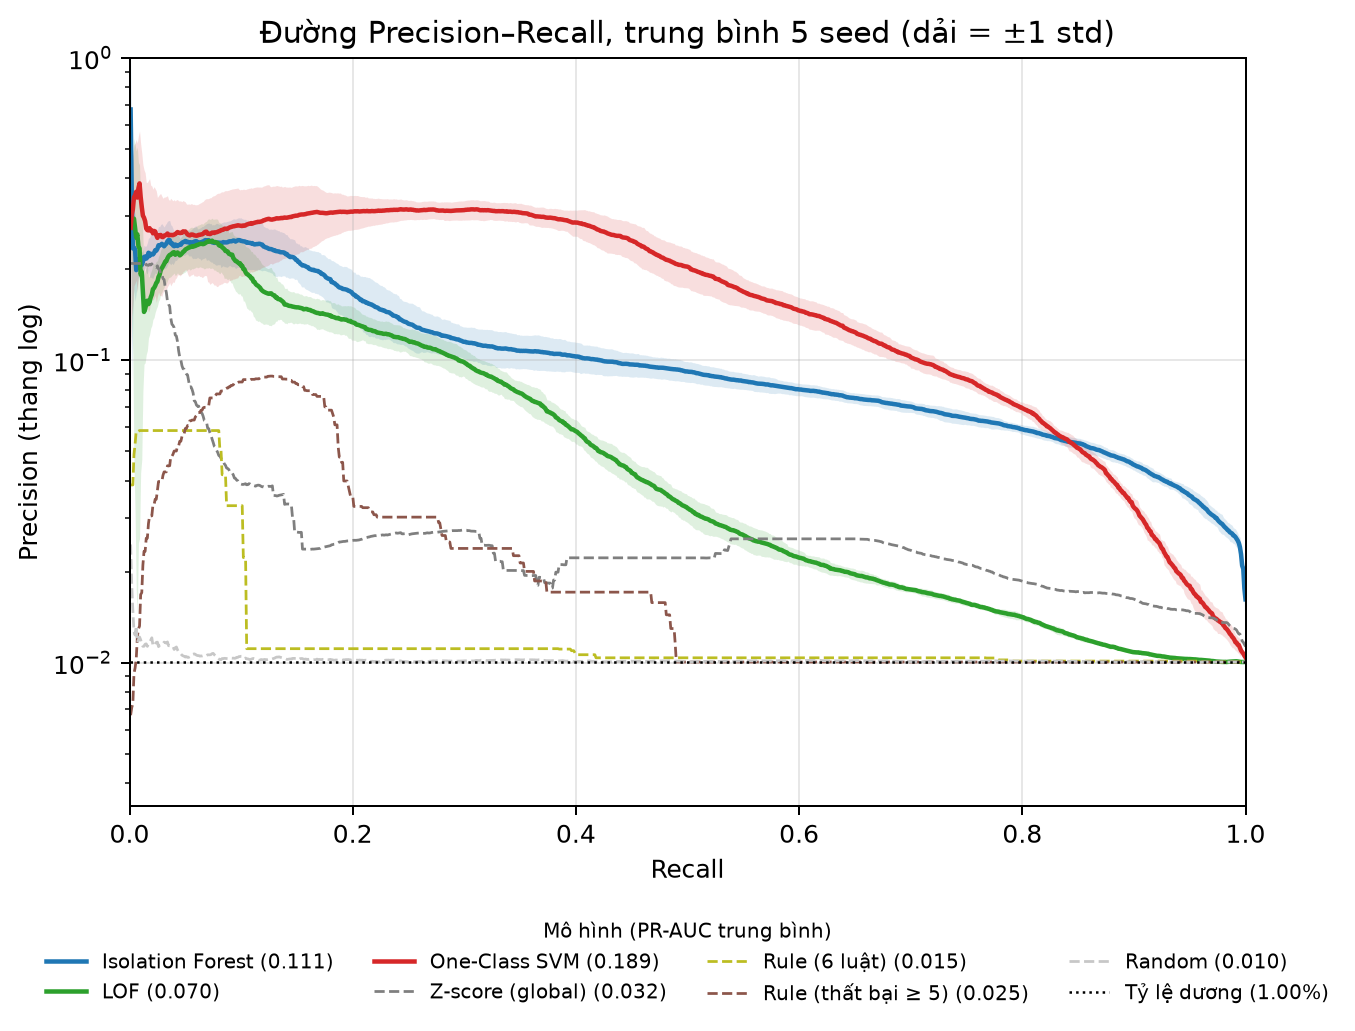
\includegraphics{../../../experiments/grid/test_22f/figures/pr_curves.png}

\textbf{Hình 4.1.} Đường precision--recall trung bình qua 5 seed
(vertical averaging, không chọn seed đẹp nhất). OCSVM giữ precision
khoảng 0,3 tới recall khoảng 0,3 rồi giảm dần; z-score có precision cao
ở vài cảnh báo đầu rồi rơi nhanh.

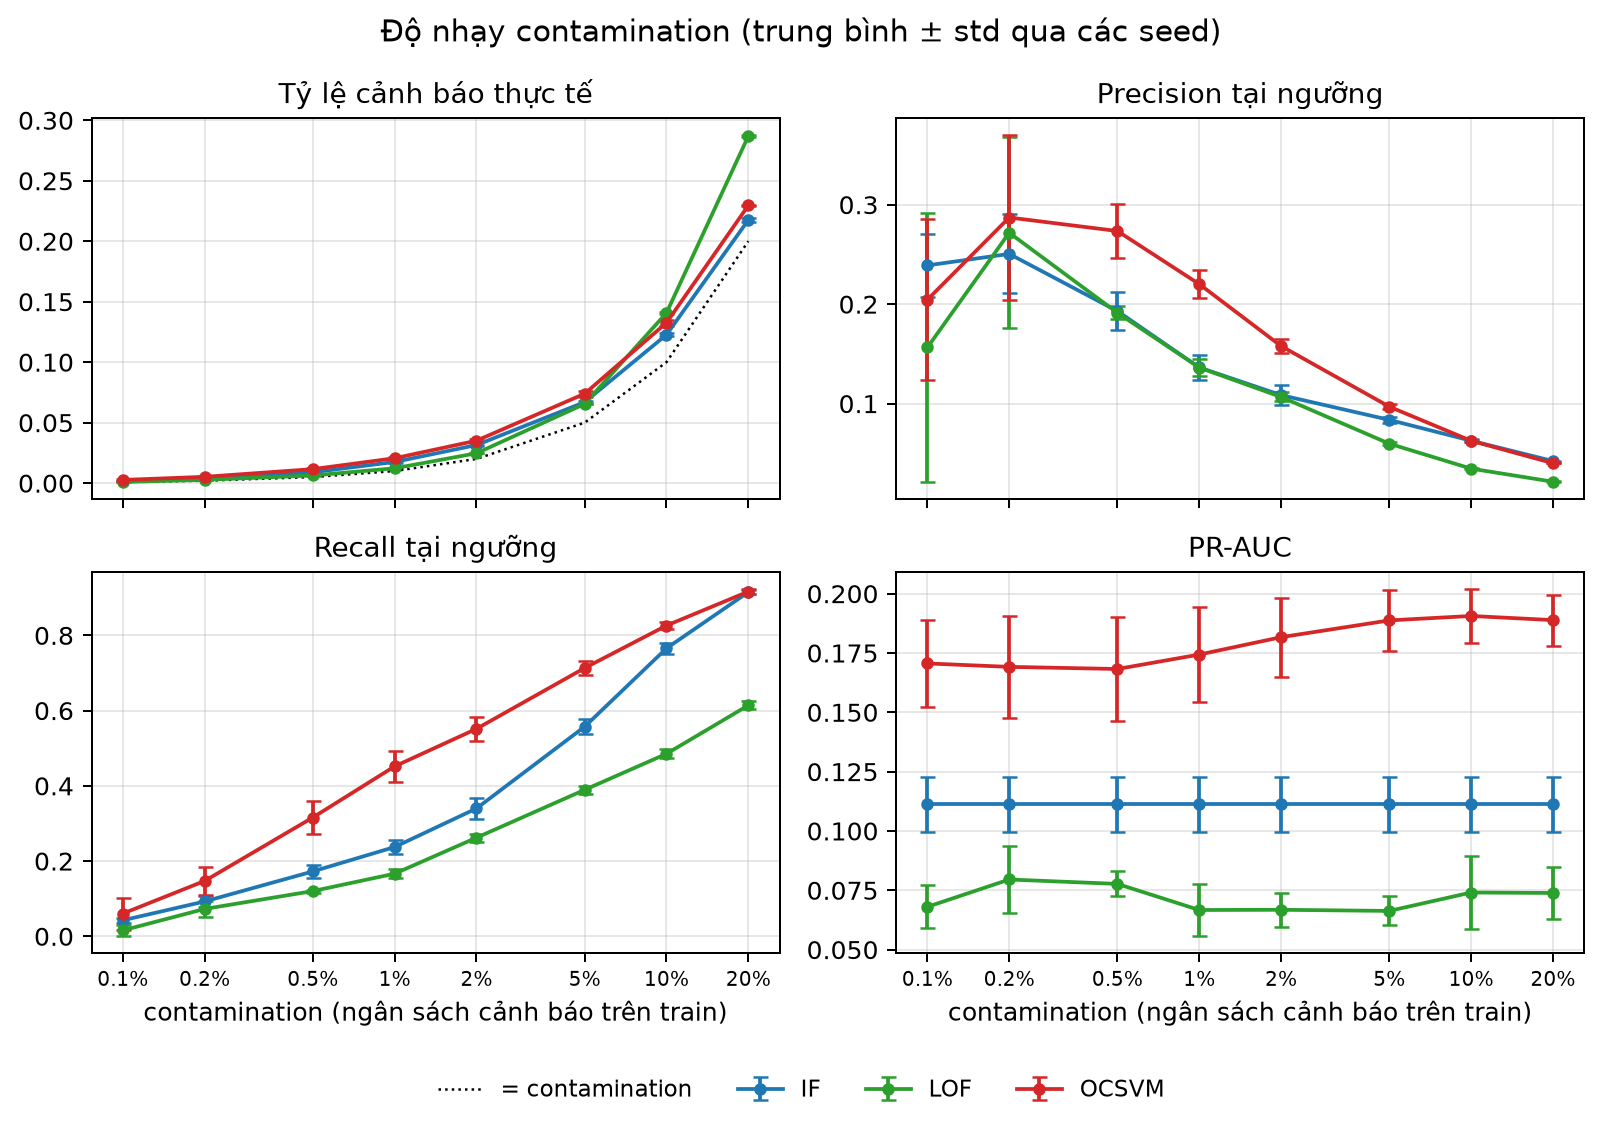
\includegraphics{../../../experiments/grid/test_22f/figures/contamination_sensitivity.png}

\textbf{Hình 4.2 và bảng 4.3: Độ nhạy contamination} (đề cương 5.6:
0,1--5\%, thêm 10\% và 20\%)

{\footnotesize\renewcommand{\small}{\footnotesize}

\begin{longtable}[]{@{}
  >{\raggedright\arraybackslash}p{(\columnwidth - 10\tabcolsep) * \real{0.1011}}
  >{\raggedright\arraybackslash}p{(\columnwidth - 10\tabcolsep) * \real{0.1187}}
  >{\raggedright\arraybackslash}p{(\columnwidth - 10\tabcolsep) * \real{0.1187}}
  >{\raggedright\arraybackslash}p{(\columnwidth - 10\tabcolsep) * \real{0.1187}}
  >{\raggedright\arraybackslash}p{(\columnwidth - 10\tabcolsep) * \real{0.2649}}
  >{\raggedright\arraybackslash}p{(\columnwidth - 10\tabcolsep) * \real{0.2578}}@{}}
\toprule\noalign{}
\begin{minipage}[b]{\linewidth}\raggedright
c
\end{minipage} & \begin{minipage}[b]{\linewidth}\raggedright
OCSVM P / R
\end{minipage} & \begin{minipage}[b]{\linewidth}\raggedright
IF P / R
\end{minipage} & \begin{minipage}[b]{\linewidth}\raggedright
LOF P / R
\end{minipage} & \begin{minipage}[b]{\linewidth}\raggedright
Tỷ lệ cảnh báo thực tế (OCSVM)
\end{minipage} & \begin{minipage}[b]{\linewidth}\raggedright
Cảnh báo/ngày (OCSVM, khoảng)
\end{minipage} \\
\midrule\noalign{}
\endhead
\bottomrule\noalign{}
\endlastfoot
0,1\% & 0,30 / 0,09 & 0,24 / 0,04 & 0,19 / 0,02 & 0,3\% & 25 \\
0,2\% & 0,31 / 0,16 & 0,25 / 0,09 & 0,22 / 0,05 & 0,5\% & 40 \\
0,5\% & 0,26 / 0,31 & 0,19 / 0,17 & 0,18 / 0,11 & 1,2\% & 100 \\
1\% & 0,21 / 0,41 & 0,14 / 0,24 & 0,14 / 0,17 & 1,9\% & 160 \\
2\% & 0,16 / 0,52 & 0,11 / 0,34 & 0,11 / 0,27 & 3,3\% & 280 \\
5\% & 0,10 / 0,68 & 0,08 / 0,56 & 0,06 / 0,40 & 6,9\% & 590 \\
\end{longtable}

}

\begin{itemize}
\tightlist
\item
  \textbf{Contamination chỉ dời điểm vận hành, không đổi chất lượng xếp
  hạng:} PR-AUC OCSVM chỉ dao động 0,174--0,181 dù \texttt{nu} đổi theo
  contamination; IF và LOF chỉ đổi ngưỡng.
\item
  \textbf{Chọn contamination là chọn ngân sách analyst.} Ở c = 0,5\%,
  OCSVM bật khoảng 100 cảnh báo/ngày (khoảng 8.500 dòng User/ngày), cứ
  khoảng 4 cảnh báo có 1 tấn công, bắt khoảng 31\% nạn nhân.
\item
  \textbf{Tỷ lệ cảnh báo thực tế cao hơn contamination 1,4--2,5 lần} vì
  khối chấm có thêm 1\% dương và hành vi trôi so với train. Ngưỡng đặt
  theo phân vị train không giữ đúng ngân sách khi dữ liệu trôi; cần theo
  dõi khi triển khai.
\end{itemize}

\hypertarget{theo-loux1ea1i-tux1ea5n-cuxf4ng}{%
\subsection{4.4. Theo loại tấn
công}\label{theo-loux1ea1i-tux1ea5n-cuxf4ng}}

\textbf{Bảng 4.4: ROC-AUC theo kịch bản, test, 22 đặc trưng, TB 5 run}

{\footnotesize\renewcommand{\small}{\footnotesize}

\begin{longtable}[]{@{}
  >{\raggedright\arraybackslash}p{(\columnwidth - 14\tabcolsep) * \real{0.2054}}
  >{\raggedright\arraybackslash}p{(\columnwidth - 14\tabcolsep) * \real{0.1043}}
  >{\raggedright\arraybackslash}p{(\columnwidth - 14\tabcolsep) * \real{0.1043}}
  >{\raggedright\arraybackslash}p{(\columnwidth - 14\tabcolsep) * \real{0.1043}}
  >{\raggedright\arraybackslash}p{(\columnwidth - 14\tabcolsep) * \real{0.1043}}
  >{\raggedright\arraybackslash}p{(\columnwidth - 14\tabcolsep) * \real{0.1399}}
  >{\raggedright\arraybackslash}p{(\columnwidth - 14\tabcolsep) * \real{0.1043}}
  >{\raggedright\arraybackslash}p{(\columnwidth - 14\tabcolsep) * \real{0.1134}}@{}}
\toprule\noalign{}
\begin{minipage}[b]{\linewidth}\raggedright
Kịch bản
\end{minipage} & \begin{minipage}[b]{\linewidth}\raggedright
OCSVM
\end{minipage} & \begin{minipage}[b]{\linewidth}\raggedright
IF
\end{minipage} & \begin{minipage}[b]{\linewidth}\raggedright
LOF
\end{minipage} & \begin{minipage}[b]{\linewidth}\raggedright
Z-score
\end{minipage} & \begin{minipage}[b]{\linewidth}\raggedright
Luật thất bại
\end{minipage} & \begin{minipage}[b]{\linewidth}\raggedright
Luật 6 đk
\end{minipage} & \begin{minipage}[b]{\linewidth}\raggedright
Ngẫu nhiên
\end{minipage} \\
\midrule\noalign{}
\endhead
\bottomrule\noalign{}
\endlastfoot
brute\_\allowbreak{}force & \textbf{0,992} & 0,945 & 0,581 & 0,915 &
0,988 & 0,751 & 0,500 \\
logon\_\allowbreak{}type\_\allowbreak{}switch & \textbf{0,973} & 0,967 &
0,909 & 0,791 & 0,359 & 0,406 & 0,501 \\
new\_\allowbreak{}workstation\_\allowbreak{}burst & \textbf{0,973} &
0,959 & 0,936 & 0,521 & 0,495 & 0,459 & 0,491 \\
dormant\_\allowbreak{}wakeup & 0,907 & \textbf{0,942} & 0,554 & 0,785 &
0,513 & 0,418 & 0,513 \\
off\_\allowbreak{}hours & 0,801 & \textbf{0,872} & 0,739 & 0,687 & 0,510
& 0,571 & 0,508 \\
password\_\allowbreak{}spraying & 0,709 & 0,842 & 0,586 & 0,759 &
\textbf{0,875} & 0,613 & 0,503 \\
\end{longtable}

}

ROC-AUC theo kịch bản được tính với cùng tập dòng âm. Để thấy mức ``lọt
vào ngân sách'', bảng 4.5 dùng recall top-100/ngày; bảng này đo với 41
đặc trưng và OCSVM \texttt{nc1000} (thí nghiệm phân tích theo kịch bản
tuần 5), nhưng thứ hạng kịch bản không đổi với bộ 22.

\textbf{Bảng 4.5: Recall top-100/ngày theo kịch bản, test, 41 đặc trưng,
TB 5 run}

{\footnotesize\renewcommand{\small}{\footnotesize}

\begin{longtable}[]{@{}
  >{\raggedright\arraybackslash}p{(\columnwidth - 12\tabcolsep) * \real{0.1891}}
  >{\raggedright\arraybackslash}p{(\columnwidth - 12\tabcolsep) * \real{0.0960}}
  >{\raggedright\arraybackslash}p{(\columnwidth - 12\tabcolsep) * \real{0.0960}}
  >{\raggedright\arraybackslash}p{(\columnwidth - 12\tabcolsep) * \real{0.0960}}
  >{\raggedright\arraybackslash}p{(\columnwidth - 12\tabcolsep) * \real{0.0960}}
  >{\raggedright\arraybackslash}p{(\columnwidth - 12\tabcolsep) * \real{0.1288}}
  >{\raggedright\arraybackslash}p{(\columnwidth - 12\tabcolsep) * \real{0.2780}}@{}}
\toprule\noalign{}
\begin{minipage}[b]{\linewidth}\raggedright
Kịch bản
\end{minipage} & \begin{minipage}[b]{\linewidth}\raggedright
OCSVM
\end{minipage} & \begin{minipage}[b]{\linewidth}\raggedright
IF
\end{minipage} & \begin{minipage}[b]{\linewidth}\raggedright
LOF
\end{minipage} & \begin{minipage}[b]{\linewidth}\raggedright
Z-score
\end{minipage} & \begin{minipage}[b]{\linewidth}\raggedright
Luật thất bại
\end{minipage} & \begin{minipage}[b]{\linewidth}\raggedright
Hạng trung vị của nạn nhân (OCSVM)
\end{minipage} \\
\midrule\noalign{}
\endhead
\bottomrule\noalign{}
\endlastfoot
brute\_\allowbreak{}force & \textbf{0,68} & 0,10 & 0,01 & 0,13 & 0,45 &
top 0,8\% \\
logon\_\allowbreak{}type\_\allowbreak{}switch & \textbf{0,58} & 0,42 &
0,51 & 0,02 & 0,00 & top 1,2\% \\
new\_\allowbreak{}workstation\_\allowbreak{}burst & \textbf{0,29} & 0,07
& 0,10 & 0,02 & 0,01 & top 1,8\% \\
password\_\allowbreak{}spraying & 0,19 & \textbf{0,23} & 0,04 & 0,22 &
0,05 & top 26\% \\
dormant\_\allowbreak{}wakeup & \textbf{0,17} & 0,08 & 0,08 & 0,00 & 0,04
& top 4,0\% \\
off\_\allowbreak{}hours & 0,03 & \textbf{0,08} & 0,05 & 0,06 & 0,04 &
top 7,7\% \\
\textbf{Tất cả} & \textbf{0,32} & 0,16 & 0,13 & 0,08 & 0,10 & \\
\end{longtable}

}

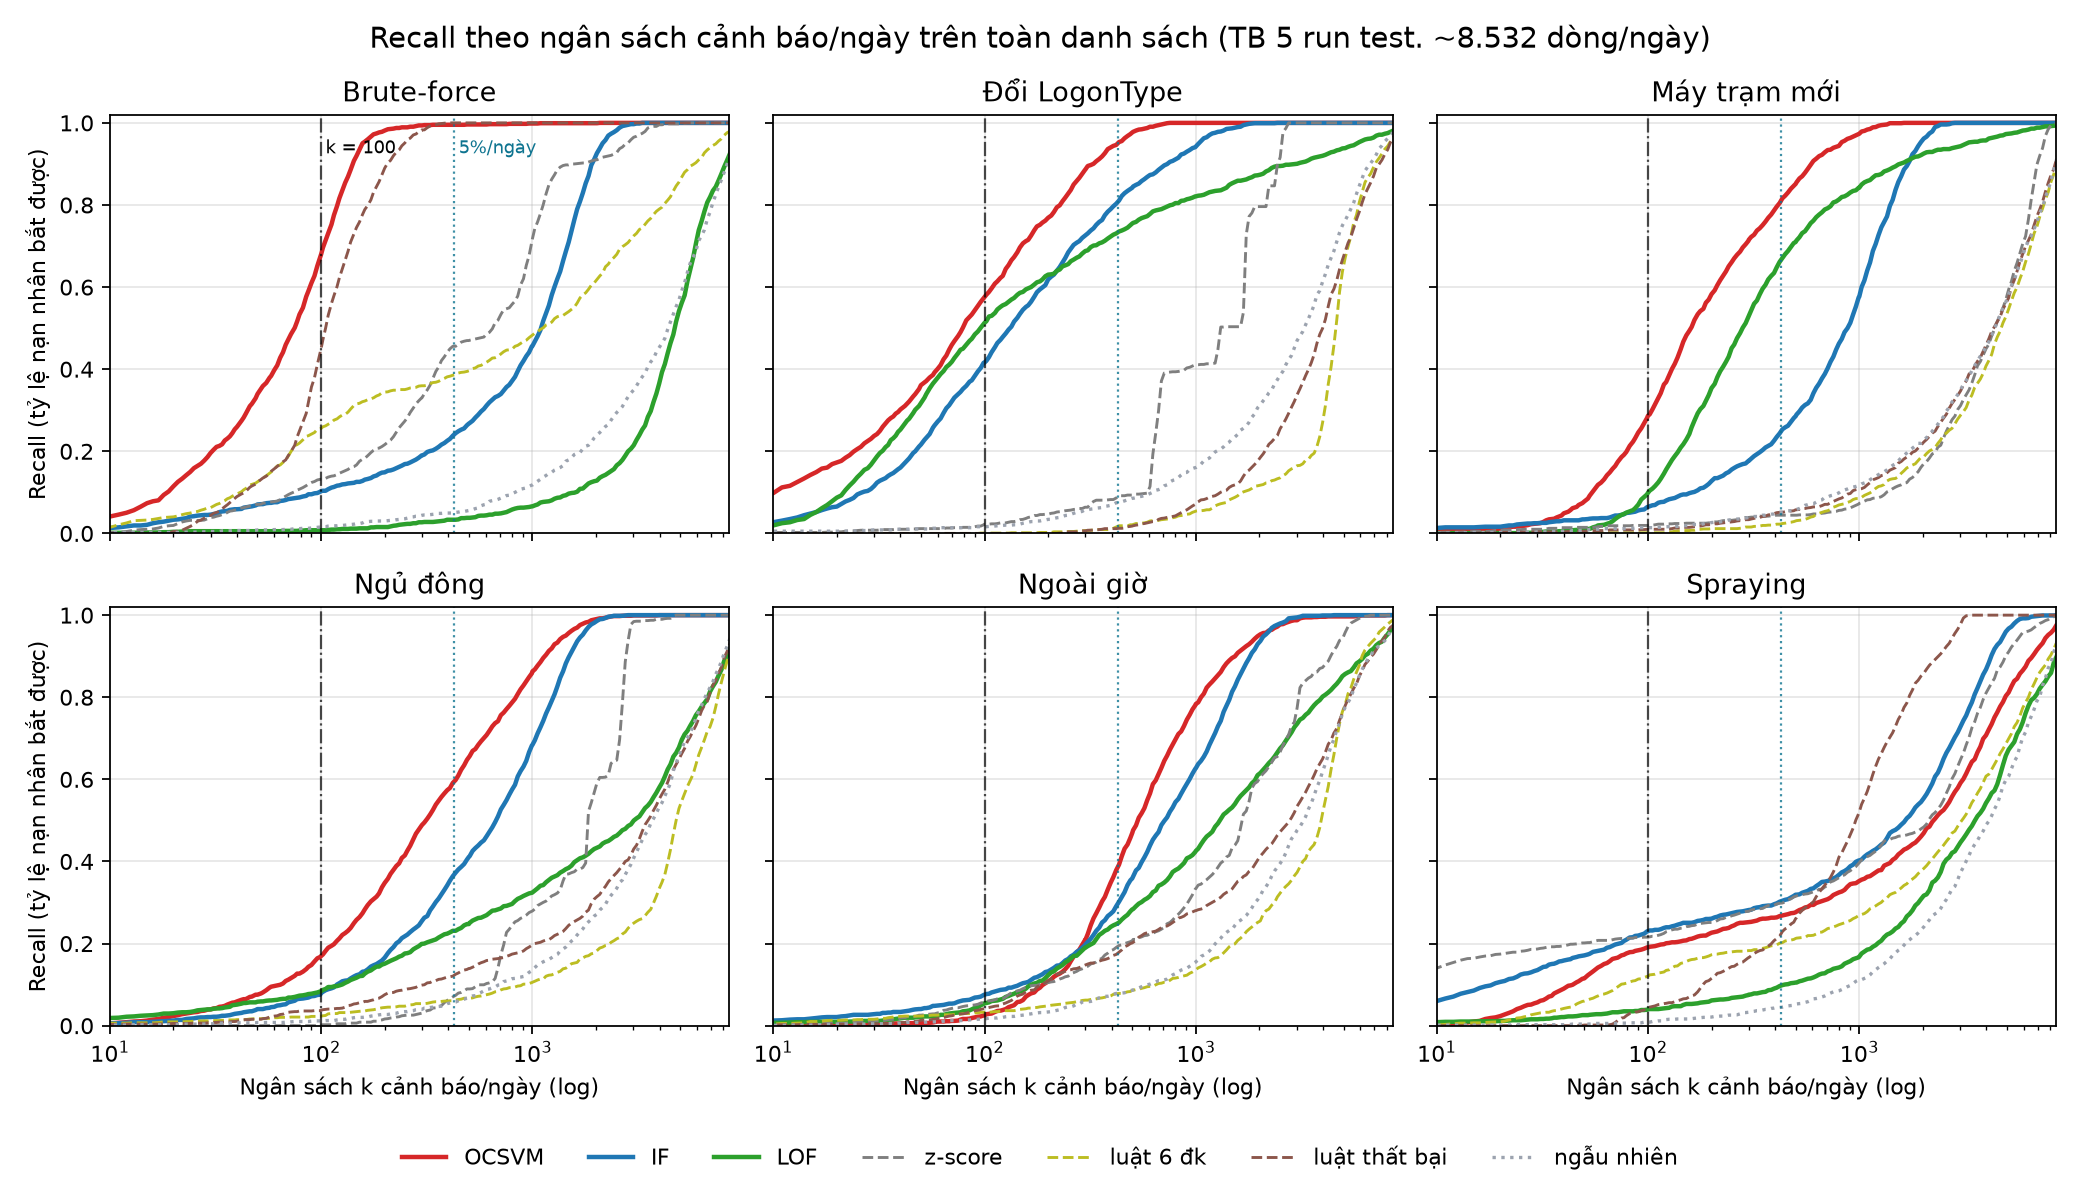
\includegraphics{../../week5/figures/03-scenario_recall_budget.png}

\textbf{Hình 4.3.} Recall theo ngân sách k cảnh báo/ngày, mỗi ô một kịch
bản (41 đặc trưng). Đường càng lên sớm càng tốt.

\textbf{Trả lời Q3:}

\begin{itemize}
\tightlist
\item
  \textbf{Bắt tốt:} brute\_\allowbreak{}force (OCSVM gần 0,7 ở 100 cảnh
  báo/ngày, gần 1,0 ở 5\%),
  logon\_\allowbreak{}type\_\allowbreak{}switch (cả ba mô hình),
  new\_\allowbreak{}workstation\_\allowbreak{}burst (chủ yếu OCSVM).
\item
  \textbf{Bắt yếu:} dormant\_\allowbreak{}wakeup; nạn nhân bị bỏ sót lại
  có \textbf{nhiều} sự kiện hơn nạn nhân bị bắt (trung vị 150 so với
  85), vì một ngày bận ``phát lại'' trông giống tài khoản bận bình
  thường.
\item
  \textbf{Điểm mù chung:} off\_\allowbreak{}hours và
  password\_\allowbreak{}spraying. Cả ba kịch bản yếu được phân tích ở
  mục 5.5.
\item
  \textbf{Không có mô hình nào thắng ở mọi kịch bản:} luật thất bại tốt
  nhất ở spraying về ROC-AUC; IF tốt hơn OCSVM ở
  dormant\_\allowbreak{}wakeup và off\_\allowbreak{}hours về ROC-AUC.
  Điều này ủng hộ việc kết hợp mô hình và luật (mục 8).
\end{itemize}

Nguồn:
\texttt{experiments/\allowbreak{}grid/\allowbreak{}test\_\allowbreak{}22f/\allowbreak{}grid\_\allowbreak{}scenarios\_\allowbreak{}summary.\allowbreak{}csv}
·
\texttt{experiments/\allowbreak{}analysis/\allowbreak{}scenario/\allowbreak{}}
·
\texttt{reports/\allowbreak{}week5/\allowbreak{}phan\_\allowbreak{}tich\_\allowbreak{}theo\_\allowbreak{}kich\_\allowbreak{}ban.\allowbreak{}md}

\hypertarget{chi-phuxed-tuxednh-touxe1n}{%
\subsection{4.5. Chi phí tính toán}\label{chi-phuxed-tuxednh-touxe1n}}

\begin{longtable}[]{@{}
  >{\raggedright\arraybackslash}p{(\columnwidth - 4\tabcolsep) * \real{0.4049}}
  >{\raggedright\arraybackslash}p{(\columnwidth - 4\tabcolsep) * \real{0.1402}}
  >{\raggedright\arraybackslash}p{(\columnwidth - 4\tabcolsep) * \real{0.4349}}@{}}
\toprule\noalign{}
\begin{minipage}[b]{\linewidth}\raggedright
Bước
\end{minipage} & \begin{minipage}[b]{\linewidth}\raggedright
Thời gian
\end{minipage} & \begin{minipage}[b]{\linewidth}\raggedright
Ghi chú
\end{minipage} \\
\midrule\noalign{}
\endhead
\bottomrule\noalign{}
\endlastfoot
Làm sạch + đặc trưng 60 ngày & vài giờ & Bước ghép lịch sử 7 ngày chiếm
phần lớn; 14 ngày tốn thêm khoảng 200 s và gần gấp đôi RAM \\
Fit OCSVM \texttt{g01} / \texttt{nc1000} & 5 s / 47 s & 315 nghìn dòng
train; \texttt{nc1000} dùng ma trận 315k × 1000 (\textgreater{} 2 GB,
biến đổi theo khối) \\
Fit IF / LOF & 12 s / 8 s & LOF HNSW đa luồng; LOF chính xác không khả
thi ở quy mô này \\
Chấm 154 nghìn dòng & 1--3 s mỗi mô hình & Đủ nhanh cho chấm theo lô
hằng ngày \\
Lưới test (3 mô hình + 4 baseline × 5 seed + quét contamination) &
khoảng 1 giờ & Phần lớn là 120 lần fit của quét contamination \\
\end{longtable}

\hypertarget{phuxe2n-tuxedch}{%
\section{5. Phân tích}\label{phuxe2n-tuxedch}}

\hypertarget{vuxec-sao-ocsvm-vux1b0ux1ee3t-lof}{%
\subsection{5.1. Vì sao OCSVM vượt
LOF}\label{vuxec-sao-ocsvm-vux1b0ux1ee3t-lof}}

Nhiều bài so sánh xếp OCSVM ở nhóm kém. Kết quả ngược lại ở đây có ba
nguyên nhân:

\begin{enumerate}
\def\labelenumi{\arabic{enumi}.}
\tightlist
\item
  \textbf{Loại bất thường quyết định thuật toán thắng.} Các khảo sát lớn
  (ví dụ ADBench, NeurIPS 2022) cho thấy phương pháp toàn cục thắng với
  bất thường toàn cục, còn LOF mạnh với bất thường cục bộ. Năm trên sáu
  kịch bản ở đây là bất thường toàn cục: bị khoá tài khoản, nhiều máy
  nguồn mới, cả ngày đổi loại logon.
\item
  \textbf{Bằng chứng trực tiếp: LOF gần như mù với brute-force} (ROC-AUC
  0,58, recall top-100/ngày 0,01) trong khi OCSVM đạt 0,99. Train có sẵn
  khoảng 600 dòng User thật giống brute-force (bị khoá, ≥ 8 lần thất
  bại). Nạn nhân tiêm có láng giềng gần nhất chính là các dòng này, mật
  độ tương đương nên LOF ≈ 1, tức ``bình thường''. OCSVM đo khoảng cách
  tới khối dữ liệu chính; 600 trên 315.000 dòng là vùng thưa nên bị coi
  là bất thường.
\item
  \textbf{Tiền xử lý quyết định} (mục 5.2).
\end{enumerate}

\hypertarget{scaler-lux1ef1a-chux1ecdn-an-touxe0n-theo-suxe1ch-giuxe1o-khoa-cuxf3-thux1ec3-sai}{%
\subsection{5.2. Scaler: lựa chọn ``an toàn'' theo sách giáo khoa có thể
sai}\label{scaler-lux1ef1a-chux1ecdn-an-touxe0n-theo-suxe1ch-giuxe1o-khoa-cuxf3-thux1ec3-sai}}

\texttt{RobustScaler} chia mỗi đặc trưng cho IQR của train. Trên dữ liệu
UEBA, nhiều đặc trưng là tỷ lệ phần lớn bằng 0: đặc trưng có IQR rất nhỏ
bị phóng đại (\texttt{failure\_\allowbreak{}ratio} lên khoảng 1.400 đơn
vị), còn đặc trưng có IQR = 0 giữ nguyên đơn vị gốc, trong đó có chính
các đặc trưng tách nạn nhân tốt nhất. Mô hình dựa trên khoảng cách chỉ
``thấy'' vài đặc trưng bị phóng đại.

\begin{longtable}[]{@{}lll@{}}
\toprule\noalign{}
OCSVM, dev, 22 đặc trưng & Recall top-100/ngày & PR-AUC \\
\midrule\noalign{}
\endhead
\bottomrule\noalign{}
\endlastfoot
RobustScaler & 0,094 & 0,033 \\
QuantileTransformer & 0,174 & 0,073 \\
\textbf{StandardScaler} & \textbf{0,412} & \textbf{0,239} \\
\end{longtable}

LOF thì ngược lại: RobustScaler tốt nhất (0,078 so với 0,014 PR-AUC), vì
nó bắt mạnh vài kịch bản có đặc trưng bị phóng đại. Isolation Forest
không bị ảnh hưởng vì không phụ thuộc thang đo. \textbf{Bài học:} cần
kiểm tra thang đo sau tiền xử lý trước khi kết luận một mô hình kém.

\hypertarget{chux1ecdn-ux111ux1eb7c-trux1b0ng-tux1eeb-41-xuux1ed1ng-22}{%
\subsection{5.3. Chọn đặc trưng: từ 41 xuống
22}\label{chux1ecdn-ux111ux1eb7c-trux1b0ng-tux1eeb-41-xuux1ed1ng-22}}

\hypertarget{shap-muxf4-huxecnh-duxf9ng-ux111uxfang-tuxedn-hiux1ec7u}{%
\subsubsection{5.3.1. SHAP: mô hình dùng đúng tín
hiệu}\label{shap-muxf4-huxecnh-duxf9ng-ux111uxfang-tuxedn-hiux1ec7u}}

KernelSHAP trên một run dev, 180 nạn nhân (30 mỗi kịch bản) và 30 báo
nhầm điểm cao nhất của mỗi mô hình. Mỗi dòng được chuẩn hoá thành tỷ
phần \textbar SHAP\textbar{} để so giữa ba mô hình có thang điểm khác
nhau.

\begin{longtable}[]{@{}
  >{\raggedright\arraybackslash}p{(\columnwidth - 2\tabcolsep) * \real{0.4128}}
  >{\raggedright\arraybackslash}p{(\columnwidth - 2\tabcolsep) * \real{0.5672}}@{}}
\toprule\noalign{}
\begin{minipage}[b]{\linewidth}\raggedright
Kịch bản
\end{minipage} & \begin{minipage}[b]{\linewidth}\raggedright
Nhóm đặc trưng chính (tỷ phần OCSVM / IF / LOF)
\end{minipage} \\
\midrule\noalign{}
\endhead
\bottomrule\noalign{}
\endlastfoot
brute\_\allowbreak{}force & failure 0,76 / 0,51 / 0,60 \\
off\_\allowbreak{}hours & time 0,52 / 0,50 / 0,29 \\
logon\_\allowbreak{}type\_\allowbreak{}switch & logon\_\allowbreak{}type
0,44 / 0,38 / 0,22 \\
password\_\allowbreak{}spraying & failure 0,33 / 0,30 / 0,50, sau đó là
time \\
new\_\allowbreak{}workstation\_\allowbreak{}burst & novelty 0,44 / 0,34
/ 0,39 và fanout 0,35 / 0,36 / 0,18 \\
dormant\_\allowbreak{}wakeup & novelty 0,49 / 0,40 / 0,30 (chủ yếu
\texttt{days\_\allowbreak{}since\_\allowbreak{}last\_\allowbreak{}activity}) \\
\textbf{Báo nhầm} (dòng bình thường điểm cao nhất) & OCSVM:
\textbf{rhythm 0,27}; IF, LOF: failure \\
\end{longtable}

Mỗi kịch bản được giải thích bằng đúng nhóm đặc trưng thiết kế cho nó,
nhất quán ở cả ba mô hình. Nhóm \textbf{rhythm} (nhịp giữa các sự kiện)
chỉ chiếm khoảng nửa mức chia đều ở nạn nhân, nhưng chiếm 0,27 (gấp gần
3 lần mức chia đều) ở báo nhầm của OCSVM, gần như toàn bộ do
\texttt{delta\_\allowbreak{}t\_\allowbreak{}cv}. LIME được chạy để đối
chiếu nhưng khớp kém ở từng dòng (với LOF chỉ giải thích được 6\% điểm),
nên SHAP là căn cứ chính.

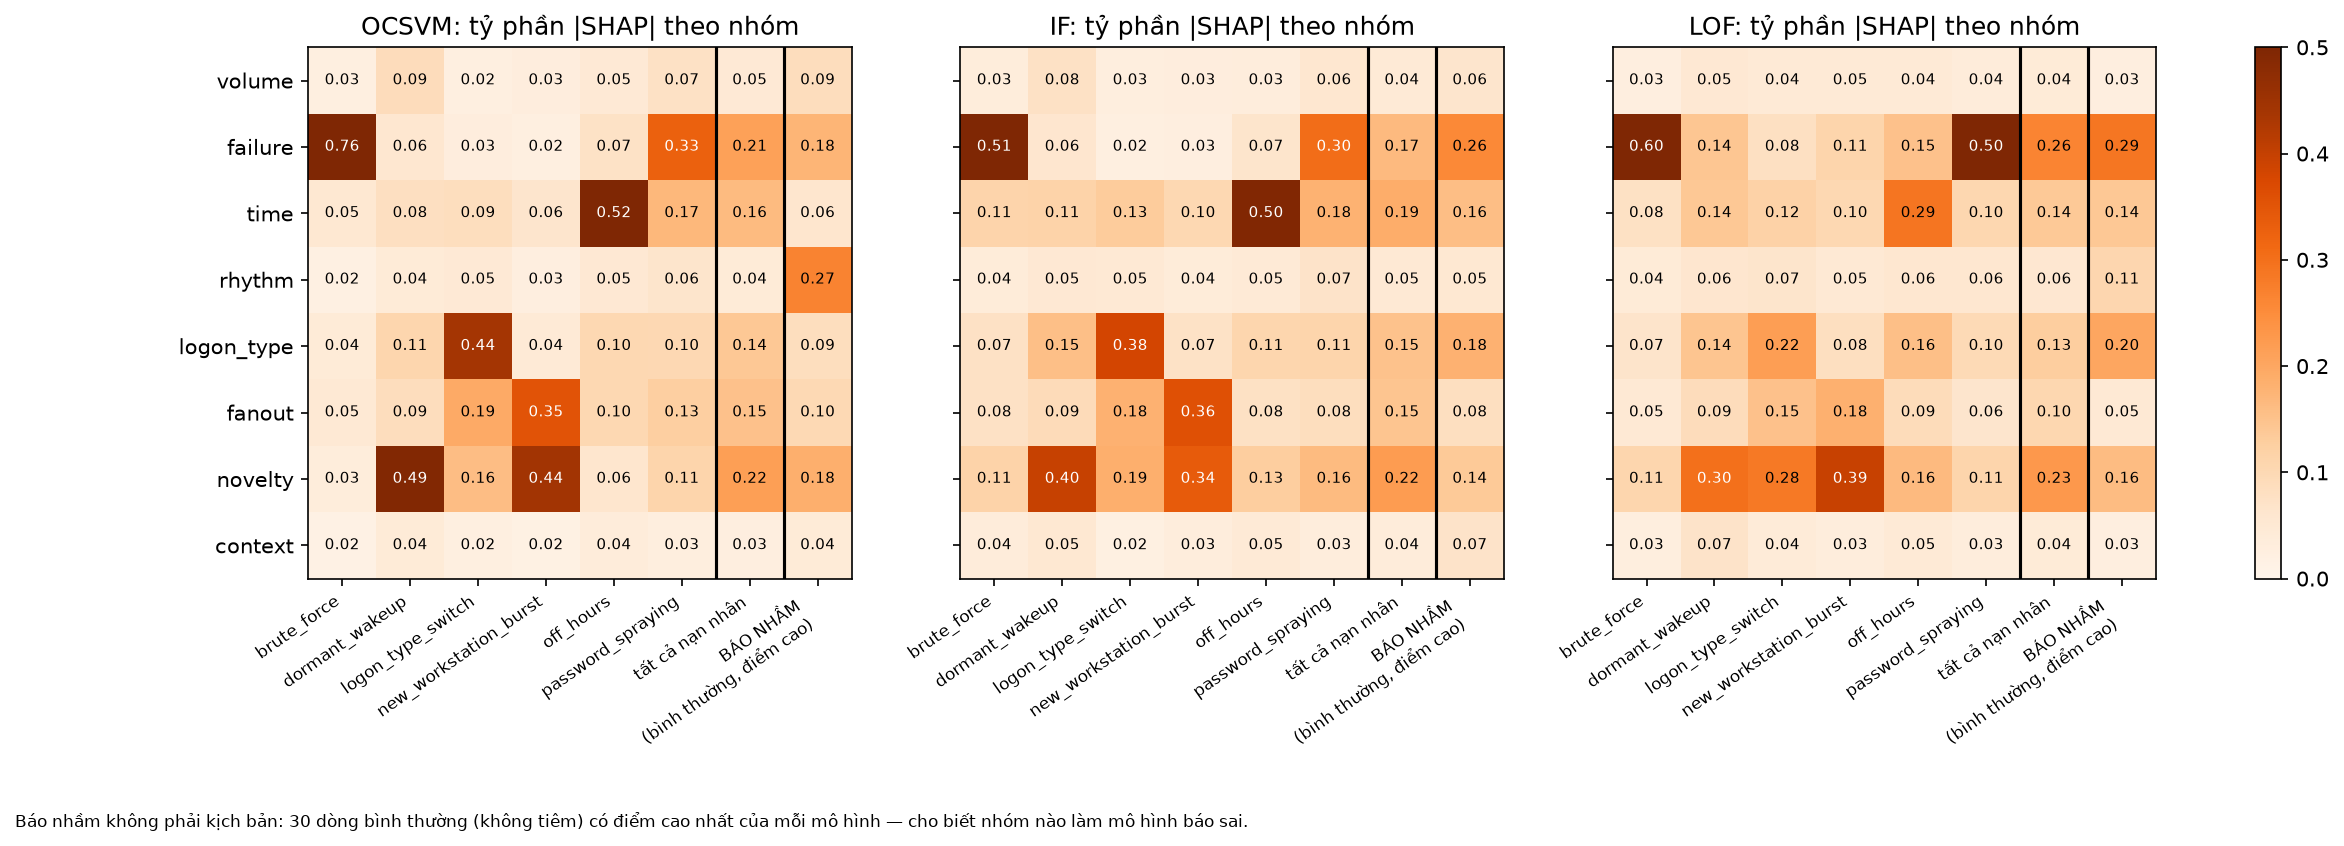
\includegraphics{../../week5/figures/04-shap_group_by_scenario.png}

\textbf{Hình 5.1.} Tỷ phần \textbar SHAP\textbar{} theo nhóm (hàng) và
kịch bản (cột), mỗi bảng một mô hình. Ô đậm gần như nằm trên một ``đường
chéo'': mỗi kịch bản có đúng một nhóm nổi bật.

\hypertarget{ablation-theo-nhuxf3m-ux111ux1eb7c-trux1b0ng-ux111ux1ec1-cux1b0ux1a1ng-5.6}{%
\subsubsection{5.3.2. Ablation theo nhóm đặc trưng (đề cương
5.6)}\label{ablation-theo-nhuxf3m-ux111ux1eb7c-trux1b0ng-ux111ux1ec1-cux1b0ux1a1ng-5.6}}

Bỏ lần lượt từng nhóm, đo hiệu ghép cặp so với đủ 41 đặc trưng trên cùng
run và seed (5 run dev). Đối chứng: chỉ xáo thứ tự dòng train đã làm
PR-AUC OCSVM lệch −0,020 ± 0,019 (do SGD), nên với OCSVM một thay đổi
phải vượt mức này.

\begin{longtable}[]{@{}
  >{\raggedright\arraybackslash}p{(\columnwidth - 8\tabcolsep) * \real{0.2144}}
  >{\raggedright\arraybackslash}p{(\columnwidth - 8\tabcolsep) * \real{0.1441}}
  >{\raggedright\arraybackslash}p{(\columnwidth - 8\tabcolsep) * \real{0.1101}}
  >{\raggedright\arraybackslash}p{(\columnwidth - 8\tabcolsep) * \real{0.1188}}
  >{\raggedright\arraybackslash}p{(\columnwidth - 8\tabcolsep) * \real{0.3926}}@{}}
\toprule\noalign{}
\begin{minipage}[b]{\linewidth}\raggedright
Bỏ nhóm (còn lại)
\end{minipage} & \begin{minipage}[b]{\linewidth}\raggedright
ΔPR-AUC OCSVM
\end{minipage} & \begin{minipage}[b]{\linewidth}\raggedright
ΔPR-AUC IF
\end{minipage} & \begin{minipage}[b]{\linewidth}\raggedright
ΔPR-AUC LOF
\end{minipage} & \begin{minipage}[b]{\linewidth}\raggedright
Thay đổi rõ nhất theo kịch bản
\end{minipage} \\
\midrule\noalign{}
\endhead
\bottomrule\noalign{}
\endlastfoot
failure (35) & \textbf{−0,056 ± 0,018} & −0,007 & +0,002 & OCSVM
brute\_\allowbreak{}force −0,57 recall \\
novelty (36) & −0,039 ± 0,016 & −0,018 & −0,028 & OCSVM burst −0,32; LOF
logon\_\allowbreak{}type\_\allowbreak{}switch −0,50 \\
fanout (35) & −0,014 ± 0,003 & −0,012 & +0,002 & OCSVM burst −0,14 \\
logon\_\allowbreak{}type (35) & −0,011 ± 0,005 & +0,004 & −0,012 &
logon\_\allowbreak{}type\_\allowbreak{}switch −0,14 đến −0,28 \\
time (33) & −0,002 ± 0,003 & +0,012 & −0,012 &
\textbf{off\_\allowbreak{}hours gần như không đổi} \\
volume + context (35) & +0,014 ± 0,003 & +0,038 & +0,003 & không kịch
bản nào tụt rõ \\
\textbf{rhythm (37)} & \textbf{+0,050 ± 0,013} & +0,019 & +0,029 & không
kịch bản nào tụt; brute\_\allowbreak{}force +0,13 (OCSVM) \\
\emph{đối chứng xáo dòng (41)} & \emph{−0,020 ± 0,019} & \emph{0,000} &
\emph{−0,005} & \\
\end{longtable}

\begin{itemize}
\tightlist
\item
  \textbf{failure và novelty là xương sống}; bỏ chúng làm mất đúng kịch
  bản tương ứng.
\item
  \textbf{rhythm, volume, context có hại hoặc vô ích}: bỏ đi làm cả ba
  mô hình tốt hơn.
\item
  \textbf{Bỏ nhóm time không làm off\_\allowbreak{}hours tệ đi}: các đặc
  trưng thời gian hiện có không giúp bắt kịch bản này (mục 5.5).
\end{itemize}

\hypertarget{chux1ecdn-sux1ed1-ux111ux1eb7c-trux1b0ng-bux1ecf-k}{%
\subsubsection{5.3.3. Chọn số đặc trưng bỏ
(K)}\label{chux1ecdn-sux1ed1-ux111ux1eb7c-trux1b0ng-bux1ecf-k}}

Bộ 30 đặc trưng dùng trong tuần 5 được tạo bằng cách bỏ nhóm rhythm và
\textbf{10 đặc trưng SHAP thấp nhất}. Con số 10 là một số tròn được
chọn, không có quy tắc nào đứng sau: khi xếp 41 đặc trưng theo mức đóng
góp SHAP, các giá trị giảm đều và không có chỗ gãy. Trên run dev dùng để
chọn bộ 30, hạng 10
(\texttt{same\_\allowbreak{}second\_\allowbreak{}share}) là 0,0163 và
hạng 11 (\texttt{custom\_\allowbreak{}proc\_\allowbreak{}share}) là
0,0165, chỉ chênh 0,0002; tính trung bình 3 run thì hạng 10 là 0,0164,
hạng 11 là 0,0171. Kết quả tốt của bộ 30 chỉ cho thấy bỏ các đặc trưng
đó không gây hại, chứ không chứng minh 10 là con số đúng. Vì vậy số đặc
trưng cần bỏ được chọn lại bằng \textbf{đường cong K} trên dev, với quy
tắc chọn đặt ra trước khi xem kết quả.

Xếp 41 đặc trưng theo tỷ phần \textbar SHAP\textbar{} cao nhất qua 3 mô
hình × 3 run dev; cấu hình
\texttt{drop\_\allowbreak{}rhythm\_\allowbreak{}kK} bỏ rhythm và K đặc
trưng thấp nhất. K = 18 là mức cắt tự nhiên: đúng 18 đặc trưng có tỷ
phần dưới mức chia đều 1/41 ở mọi mô hình, mọi run.

\begin{longtable}[]{@{}llll@{}}
\toprule\noalign{}
Còn lại & OCSVM & IF & LOF \\
\midrule\noalign{}
\endhead
\bottomrule\noalign{}
\endlastfoot
41 (đủ) & 0,317 ± 0,058 & 0,139 ± 0,011 & 0,165 ± 0,017 \\
37 (bỏ rhythm, K = 0) & 0,368 ± 0,057 & 0,195 ± 0,023 & 0,197 ± 0,014 \\
33 (K = 5) & 0,377 ± 0,059 & 0,217 ± 0,014 & 0,197 ± 0,018 \\
30 (rhythm + 10 SHAP thấp, bộ của tuần 5) & 0,380 ± 0,059 & 0,228 ±
0,017 & \textbf{0,207 ± 0,014} \\
29 (K = 10) & 0,380 ± 0,061 & 0,235 ± 0,022 & 0,184 ± 0,015 \\
25 (K = 15) & \textbf{0,385 ± 0,059} & 0,246 ± 0,019 & 0,181 ± 0,015 \\
\textbf{22 (K = 18, chốt)} & 0,383 ± 0,067 & \textbf{0,264 ± 0,012} &
0,170 ± 0,006 \\
21 (K = 20) & 0,382 ± 0,064 & 0,258 ± 0,021 & 0,167 ± 0,016 \\
\end{longtable}

Recall top-100/ngày, TB ± std qua 5 run dev, cấu hình mô hình của 41 đặc
trưng. Bộ 30 dùng xếp hạng SHAP của 1 run, còn đường cong K xếp theo tỷ
phần cao nhất qua 3 mô hình × 3 run, nên K = 10 cho 29 đặc trưng và
không trùng với bộ 30 (bộ 30 giữ
\texttt{custom\_\allowbreak{}proc\_\allowbreak{}share},
\texttt{delta\_\allowbreak{}mean\_\allowbreak{}distinct\_\allowbreak{}pair\_\allowbreak{}7d},
\texttt{new\_\allowbreak{}host\_\allowbreak{}count\_\allowbreak{}7d}
nhưng bỏ
\texttt{peer\_\allowbreak{}z\_\allowbreak{}share\_\allowbreak{}night},
\texttt{volume\_\allowbreak{}robust\_\allowbreak{}z\_\allowbreak{}7d}).
Nguồn:
\texttt{experiments/\allowbreak{}ablation/\allowbreak{}kcurve/\allowbreak{}summary.\allowbreak{}csv}.

\begin{itemize}
\tightlist
\item
  \textbf{OCSVM phẳng} từ 33 đến 22 đặc trưng; \textbf{IF tăng đều} tới
  22 rồi dừng; \textbf{LOF tốt nhất ở 30--33} rồi giảm.
\item
  \textbf{Không có K chung tốt nhất cho cả ba mô hình.} K = 18 được chốt
  vì là mức cắt có căn cứ, OCSVM không đổi, IF tăng rõ, và K = 20 không
  tốt hơn ở mô hình nào. Đánh đổi là LOF kém trên dev (−0,037 ± 0,009).
\item
  \textbf{Kiểm tra trên test} (bảng 5.1 của báo cáo tuần 5): so với bộ
  30, K = 18 cho OCSVM −0,003 ± 0,005, IF +0,034 ± 0,013, LOF
  \textbf{+0,028 ± 0,005} recall. LOF đảo chiều giữa dev và test, nên
  không dùng LOF để chọn K.
\item
  \textbf{Thiên lệch chọn:} K = 18 được chốt sau khi đã xem kết quả test
  của 4 cấu hình K. Với OCSVM và IF, test chỉ xác nhận dev; với LOF việc
  chọn có tính đến test. Đây là ngoại lệ duy nhất với nguyên tắc ``test
  không tham gia chọn''.
\end{itemize}

\textbf{Kết quả so với 41 đặc trưng ban đầu (test):} recall top-100/ngày
IF 0,16 → 0,24, LOF 0,13 → 0,18, OCSVM 0,32 → 0,34 (\texttt{g01};
\texttt{nc1000} 0,37). Bớt chiều yếu giúp IF nhiều nhất vì IF chọn đặc
trưng ngẫu nhiên để tách, mỗi chiều yếu làm loãng cây.

Nguồn:
\texttt{reports/\allowbreak{}week5/\allowbreak{}shap\_\allowbreak{}lime.\allowbreak{}md}
·
\texttt{ablation\_\allowbreak{}nhom\_\allowbreak{}dac\_\allowbreak{}trung.\allowbreak{}md}
·
\texttt{chon\_\allowbreak{}so\_\allowbreak{}dac\_\allowbreak{}trung\_\allowbreak{}K.\allowbreak{}md}
·
\texttt{kiem\_\allowbreak{}tra\_\allowbreak{}test\_\allowbreak{}K\_\allowbreak{}va\_\allowbreak{}context.\allowbreak{}md}

\hypertarget{cux1eeda-sux1ed5-lux1ecbch-sux1eed-7-14-21-nguxe0y}{%
\subsection{5.4. Cửa sổ lịch sử 7 / 14 / 21
ngày}\label{cux1eeda-sux1ed5-lux1ecbch-sux1eed-7-14-21-nguxe0y}}

Kéo dài cửa sổ của các đặc trưng lịch sử \textbf{không cải thiện} kết
quả: recall top-100/ngày OCSVM 0,317 / 0,318 / 0,294; LOF 0,121 / 0,034
/ 0,003 (sụp ở cửa sổ dài vì nhiều dòng đầu train thiếu lịch sử bị điền
median, tạo cụm dày giả). Cửa sổ dài chỉ giúp spraying (ROC-AUC 0,69 →
0,77) nhưng làm hại dormant\_\allowbreak{}wakeup và tốn khoảng 3 lần
thời gian. \textbf{Giữ 7 ngày.} Chi tiết:
\texttt{reports/\allowbreak{}week5/\allowbreak{}bao\_\allowbreak{}cao\_\allowbreak{}tuan5.\allowbreak{}md}
mục 1.

\hypertarget{ba-kux1ecbch-bux1ea3n-bux1ecb-bux1eaft-kuxe9m-off_hours-password_spraying-dormant_wakeup}{%
\subsection{\texorpdfstring{5.5. Ba kịch bản bị bắt kém:
off\_\allowbreak{}hours, password\_\allowbreak{}spraying,
dormant\_\allowbreak{}wakeup}{5.5. Ba kịch bản bị bắt kém:   }}\label{ba-kux1ecbch-bux1ea3n-bux1ecb-bux1eaft-kuxe9m-off_hours-password_spraying-dormant_wakeup}}

Các con số recall trong mục này lấy từ bảng 4.5 (41 đặc trưng).

\textbf{off\_\allowbreak{}hours} (recall top-100/ngày ≤ 0,08 ở mọi mô
hình):

\begin{itemize}
\tightlist
\item
  Nạn nhân bị bỏ sót có trung vị 107 sự kiện, nạn nhân bị bắt chỉ 9,5.
  Một ngày bận bị dời sang đêm vẫn trông như một tài khoản bận; trong
  không gian khoảng cách, vài chiều về ban đêm bị các chiều khối lượng
  lấn át.
\item
  SHAP xác nhận nhóm time giải thích phần lớn điểm của nạn nhân (0,52),
  nhưng điểm tuyệt đối không đủ cao để lọt top.
\item
  \textbf{Khung giờ đêm quá rộng.} Ngoài giờ là 18h--7h, tức 14/24 giờ,
  và chứa cả 7h, lúc lưu lượng ngày thường đã bằng 90\% giờ cao điểm
  (mục 2.5). Một ngày bị dời vào khung này vì vậy không khác nhiều so
  với một ngày bình thường.
\item
  \textbf{Nhóm đặc trưng thời gian hiện không tạo khác biệt:} bỏ cả 8
  đặc trưng thời gian thì recall off\_\allowbreak{}hours gần như không
  đổi ở cả 3 mô hình (−0,02 đến 0,00).
\item
  \textbf{Không phải do lệch múi giờ:} nhịp lưu lượng theo giờ khớp với
  giờ địa phương (mục 2.5).
\item
  Hướng sửa: thu hẹp khung giờ đêm, và dùng đặc trưng so giờ hoạt động
  với \textbf{lịch sử giờ của chính tài khoản}, hoặc một luật riêng.
\end{itemize}

\textbf{password\_\allowbreak{}spraying} (recall ≤ 0,23):

\begin{itemize}
\tightlist
\item
  Mỗi nạn nhân chỉ nhận 1--3 lần thử. Ở mức (tài khoản, ngày) gần như
  không có tín hiệu; dấu hiệu thật là \textbf{một máy nguồn làm nhiều
  tài khoản thất bại trong thời gian ngắn}, nhưng mọi đặc trưng đều tính
  theo từng tài khoản.
\item
  Luật thất bại có ROC-AUC tốt nhất (0,875) nhưng vẫn không đưa được nạn
  nhân vào top (recall 0,05).
\item
  Hướng sửa: đặc trưng \textbf{fan-out theo máy nguồn} (engine đã có
  phép đo \texttt{fanout}), hoặc phân tích ở cấp máy nguồn thay vì cấp
  tài khoản. Không chỉnh tham số mô hình nào giải được vấn đề này.
\end{itemize}

\textbf{dormant\_\allowbreak{}wakeup} (recall ≤ 0,17; ROC-AUC 0,91 với
OCSVM và 0,94 với IF):

\begin{itemize}
\tightlist
\item
  Bộ tiêm phát lại một ngày bình thường của chính tài khoản sau một
  khoảng nghỉ dài. Chỉ có khoảng nghỉ là khác thường; khối lượng, máy và
  loại đăng nhập đều giống một ngày bình thường.
\item
  Nạn nhân bị bỏ sót lại có \textbf{nhiều} sự kiện hơn nạn nhân bị bắt
  (trung vị 150 so với 85), vì một ngày bận trông giống một tài khoản
  bận bình thường.
\item
  Tín hiệu rõ nhất chỉ còn
  \texttt{days\_\allowbreak{}since\_\allowbreak{}last\_\allowbreak{}activity}.
  Sau khoảng nghỉ từ 7 ngày trở lên, các đặc trưng so với 7 ngày trước
  không có lịch sử để so (suy luận từ cách tính, chưa đo riêng).
\item
  Hướng sửa: đặc trưng ``khoảng nghỉ hôm nay so với khoảng nghỉ dài nhất
  trước đó của chính tài khoản''.
\end{itemize}

\textbf{Nguyên nhân chung.} Cả ba kịch bản đều chạm vào giới hạn của
cách đặt bài toán: \textbf{mỗi dòng là một tài khoản trong một ngày}.
Spraying cần nhìn theo máy nguồn qua nhiều tài khoản;
off\_\allowbreak{}hours và dormant\_\allowbreak{}wakeup cần so với lịch
sử dài hơn của chính tài khoản. Chỉnh tham số mô hình không giải được
các điểm mù này.

\hypertarget{ux111ux1ed9-ux1ed5n-ux111ux1ecbnh}{%
\subsection{5.6. Độ ổn định}\label{ux111ux1ed9-ux1ed5n-ux111ux1ecbnh}}

\textbf{Qua seed.} Std của recall top-100/ngày: IF 0,016, LOF 0,006,
OCSVM \texttt{g01} 0,070. Std gồm cả biến động dữ liệu tiêm và mô hình.
Riêng OCSVM còn nhạy với thứ tự dòng train (SGD), nên dòng được sắp cố
định trước khi fit.

\textbf{Chọn cấu hình OCSVM trên dev không lặp lại trên test.} Trên dev,
\texttt{g01} thắng \texttt{nc1000} với mức chênh nhỏ hơn 1 std. Trên
test:

\begin{longtable}[]{@{}
  >{\raggedright\arraybackslash}p{(\columnwidth - 6\tabcolsep) * \real{0.3415}}
  >{\raggedright\arraybackslash}p{(\columnwidth - 6\tabcolsep) * \real{0.2976}}
  >{\raggedright\arraybackslash}p{(\columnwidth - 6\tabcolsep) * \real{0.1448}}
  >{\raggedright\arraybackslash}p{(\columnwidth - 6\tabcolsep) * \real{0.1961}}@{}}
\toprule\noalign{}
\begin{minipage}[b]{\linewidth}\raggedright
OCSVM, test
\end{minipage} & \begin{minipage}[b]{\linewidth}\raggedright
PR-AUC từng run
\end{minipage} & \begin{minipage}[b]{\linewidth}\raggedright
TB ± std
\end{minipage} & \begin{minipage}[b]{\linewidth}\raggedright
Recall top-100/ngày
\end{minipage} \\
\midrule\noalign{}
\endhead
\bottomrule\noalign{}
\endlastfoot
\texttt{g01} (300 thành phần Nystroem, γ = 0,1) & 0,19 / 0,20 /
\textbf{0,11} / 0,15 / 0,24 & 0,175 ± 0,048 & 0,336 ± 0,070 \\
\texttt{nc1000} (1.000 thành phần, γ = scale) & 0,19 / 0,19 / 0,17 /
0,20 / 0,20 & 0,189 ± 0,013 & 0,373 ± 0,022 \\
\end{longtable}

Chênh lệch trung bình nằm trong 1 std, nhưng \texttt{g01} dao động gấp
khoảng 3--4 lần. Nhiều thành phần Nystroem hơn làm xấp xỉ nhân RBF ổn
định hơn. Kết quả chính vẫn báo cáo \texttt{g01} (cấu hình chọn trên
dev), vì đổi sang \texttt{nc1000} sau khi xem test là chọn mô hình bằng
tập test. Đề cương ghi ``một mô hình có phương sai lớn giữa các seed là
mô hình không đáng tin để triển khai''; vì vậy khuyến nghị triển khai là
\texttt{nc1000} (mục 8), và quy tắc chọn cấu hình về sau nên xét cả
trung bình lẫn độ lệch chuẩn trên dev.

\textbf{LOF không tất định.} Chỉ mục HNSW dựng đa luồng
(\texttt{n\_\allowbreak{}jobs: -1}) đổi thứ tự chèn mỗi lần fit:

\begin{itemize}
\tightlist
\item
  Trung bình 5 run lặp lại được: hai lần chạy lưới test cho recall 0,176
  và 0,175, PR-AUC 0,070 và 0,071.
\item
  Nhưng \textbf{từng lần fit} lệch nhiều: PR-AUC của run seed 42 là
  0,072 / 0,075 / 0,079 / 0,083 qua bốn lần fit (lệch tới khoảng 15\%),
  và top 50 cảnh báo của hai lần fit trên log gốc chỉ trùng
  \textbf{6/50}.
\item
  Hệ quả: danh sách cảnh báo của LOF không tái lập được. Đặt
  \texttt{n\_\allowbreak{}jobs: 1} cho kết quả tất định nhưng fit chậm
  hơn nhiều; nhóm giữ đa luồng và ghi nhận đây là hạn chế.
\end{itemize}

\hypertarget{mux1ee9c-lux1ea1c-quan-cux1ee7a-kux1ebft-quux1ea3}{%
\subsection{5.7. Mức lạc quan của kết
quả}\label{mux1ee9c-lux1ea1c-quan-cux1ee7a-kux1ebft-quux1ea3}}

\begin{itemize}
\tightlist
\item
  \textbf{Do chọn cấu hình trên dev:} nhỏ. Dev nằm trong train; với cấu
  hình 41 đặc trưng, PR-AUC test bằng hoặc cao hơn dev ở cả ba mô hình.
  Với 22 đặc trưng, PR-AUC test thấp hơn dev (OCSVM 0,175 so với 0,248),
  một phần do dev và test khác nhau về độ dài train và số ngày chấm.
\item
  \textbf{Do nhãn tổng hợp:} lớn và không đo được. Tấn công tiêm là bản
  sao sự kiện thật nhưng theo khuôn cố định; tấn công thật đa dạng và
  kín đáo hơn. Mọi con số trong báo cáo là cận trên.
\end{itemize}

\hypertarget{ux111uxe1nh-giuxe1-ux111ux1ecbnh-tuxednh-review-thux1ee7-cuxf4ng-top-50}{%
\section{6. Đánh giá định tính: review thủ công top
50}\label{ux111uxe1nh-giuxe1-ux111ux1ecbnh-tuxednh-review-thux1ee7-cuxf4ng-top-50}}

\hypertarget{thiux1ebft-lux1eadp}{%
\subsection{6.1. Thiết lập}\label{thiux1ebft-lux1eadp}}

Trên \textbf{log gốc, không tiêm}, mô hình fit ngày 1--42 và chấm ngày
43--60 (phân khúc User, seed 42). Lấy 50 cảnh báo điểm cao nhất của mỗi
mô hình, hợp lại, xáo thứ tự và \textbf{làm mù} (phiếu chấm không có tên
mô hình hay điểm; bảng khoá để riêng). Mỗi cảnh báo có một ``thẻ'' gồm
đặc trưng lệch nhất so với train, ngữ cảnh tài khoản và tóm tắt log thô
của ngày đó. Ba nhãn theo đề cương 5.5: \textbf{a} đáng ngờ, cần điều
tra; \textbf{b} bất thường nhưng giải thích được; \textbf{c} nhiễu.
Hướng dẫn chấm:
\texttt{docs/\allowbreak{}huong\_\allowbreak{}dan\_\allowbreak{}review\_\allowbreak{}top50.\allowbreak{}md}.

\hypertarget{trux1ea1ng-thuxe1i}{%
\subsection{6.2. Trạng thái}\label{trux1ea1ng-thuxe1i}}

\begin{longtable}[]{@{}
  >{\raggedright\arraybackslash}p{(\columnwidth - 8\tabcolsep) * \real{0.1904}}
  >{\raggedright\arraybackslash}p{(\columnwidth - 8\tabcolsep) * \real{0.2545}}
  >{\raggedright\arraybackslash}p{(\columnwidth - 8\tabcolsep) * \real{0.1411}}
  >{\raggedright\arraybackslash}p{(\columnwidth - 8\tabcolsep) * \real{0.2633}}
  >{\raggedright\arraybackslash}p{(\columnwidth - 8\tabcolsep) * \real{0.1307}}@{}}
\toprule\noalign{}
\begin{minipage}[b]{\linewidth}\raggedright
Bộ
\end{minipage} & \begin{minipage}[b]{\linewidth}\raggedright
Mô hình
\end{minipage} & \begin{minipage}[b]{\linewidth}\raggedright
Số cảnh báo
\end{minipage} & \begin{minipage}[b]{\linewidth}\raggedright
Người chấm
\end{minipage} & \begin{minipage}[b]{\linewidth}\raggedright
Trạng thái
\end{minipage} \\
\midrule\noalign{}
\endhead
\bottomrule\noalign{}
\endlastfoot
\textbf{\texttt{review\_\allowbreak{}top50\_\allowbreak{}22f}} &
\textbf{22 đặc trưng, OCSVM \texttt{g01}} & \textbf{148} & \textbf{2
thực tập sinh, độc lập} & \textbf{Chưa chấm} \\
\end{longtable}

\begin{quote}
Một phần \textbf{Mục này chưa hoàn chỉnh.} Đề cương yêu cầu hai thực tập
sinh chấm độc lập rồi đo đồng thuận (Cohen's κ, chạy
\texttt{python scripts/\allowbreak{}evaluation/\allowbreak{}review\_\allowbreak{}agreement.\allowbreak{}py}).
Khi có nhãn của hai người, mục này cần bổ sung bảng phân loại a/b/c theo
mô hình, κ và nhận xét.
\end{quote}

Nguồn:
\texttt{experiments/\allowbreak{}analysis/\allowbreak{}review\_\allowbreak{}top50\_\allowbreak{}22f/\allowbreak{}}

\hypertarget{hux1ea1n-chux1ebf-ux111uxe3-biux1ebft}{%
\section{7. Hạn chế đã
biết}\label{hux1ea1n-chux1ebf-ux111uxe3-biux1ebft}}

\begin{enumerate}
\def\labelenumi{\arabic{enumi}.}
\tightlist
\item
  \textbf{Nhãn tổng hợp cho cận trên lạc quan.} Tấn công thật đa dạng và
  kín đáo hơn khuôn tiêm; dòng nhãn 0 cũng chưa chắc lành tính. Không có
  nhãn tấn công thật để hiệu chỉnh.
\item
  \textbf{Giả định train ``sạch'' không hoàn toàn đúng.} Train có khoảng
  600 dòng giống brute-force thật; chính chúng làm LOF thất bại.
\item
  \textbf{Chỉ đánh giá phân khúc User.} Tài khoản Machine không được
  tiêm; Admin, Service, System quá ít để học máy.
\item
  \textbf{Ba kịch bản bị bắt kém: password\_\allowbreak{}spraying,
  off\_\allowbreak{}hours, dormant\_\allowbreak{}wakeup} (recall
  top-100/ngày ≤ 0,23 / 0,08 / 0,17, số của 41 đặc trưng). Nguyên nhân:
  (a) đặc trưng chỉ tính theo từng tài khoản, nên không thấy một máy
  nguồn thử nhiều tài khoản; (b) khung giờ đêm 18h--7h quá rộng, chứa cả
  giờ làm việc lúc 7h; (c) ngày ``thức dậy'' giống một ngày bình thường,
  chỉ khác khoảng nghỉ. Chi tiết và hướng sửa ở mục 5.5.
\item
  \textbf{Thuật toán xấp xỉ.} LOF dùng láng giềng xấp xỉ HNSW, OCSVM
  dùng nhân RBF xấp xỉ Nystroem + SGD, thay cho bản chính xác của
  scikit-learn. Kết luận về ``LOF'' và ``OCSVM'' là kết luận về các bản
  xấp xỉ này.
\item
  \textbf{LOF không tất định} ở mức từng lần fit (mục 5.6); danh sách
  cảnh báo LOF không tái lập được.
\item
  \textbf{OCSVM \texttt{g01} kém ổn định} trên test; quy tắc chọn chỉ
  dựa trên trung bình.
\item
  \textbf{Thiên lệch chọn ở bước chọn K} (mục 5.3.3): K = 18 được chốt
  sau khi xem test.
\item
  \textbf{Train dùng chung cho mọi run:} chỉ ngày chấm bị tiêm, nên độ
  lệch chuẩn không gồm biến động của train.
\item
  \textbf{Ngưỡng theo phân vị train không giữ ngân sách} khi hành vi
  trôi: tỷ lệ cảnh báo thực tế cao hơn contamination 1,4--2,5 lần.
\item
  \textbf{Đổi LogonType} chỉ có 5--8 nạn nhân/run theo đúng chiều 2 →
  3/5 của đề cương.
\item
  \textbf{Review thủ công} của bộ 22 đặc trưng chưa có nhãn của hai
  người, nên báo cáo chưa có kết quả định tính trên log thật.
\item
  \textbf{Tái lập trên máy sạch chưa được thực hiện} (mục 9).
\end{enumerate}

\hypertarget{khuyux1ebfn-nghux1ecb-triux1ec3n-khai}{%
\section{8. Khuyến nghị triển
khai}\label{khuyux1ebfn-nghux1ecb-triux1ec3n-khai}}

\hypertarget{kiux1ebfn-truxfac-phuxe2n-luux1ed3ng-theo-loux1ea1i-tuxe0i-khoux1ea3n}{%
\subsection{8.1. Kiến trúc phân luồng theo loại tài
khoản}\label{kiux1ebfn-truxfac-phuxe2n-luux1ed3ng-theo-loux1ea1i-tuxe0i-khoux1ea3n}}

\begin{longtable}[]{@{}
  >{\raggedright\arraybackslash}p{(\columnwidth - 4\tabcolsep) * \real{0.2436}}
  >{\raggedright\arraybackslash}p{(\columnwidth - 4\tabcolsep) * \real{0.2565}}
  >{\raggedright\arraybackslash}p{(\columnwidth - 4\tabcolsep) * \real{0.4798}}@{}}
\toprule\noalign{}
\begin{minipage}[b]{\linewidth}\raggedright
Luồng
\end{minipage} & \begin{minipage}[b]{\linewidth}\raggedright
Đối tượng
\end{minipage} & \begin{minipage}[b]{\linewidth}\raggedright
Phương pháp
\end{minipage} \\
\midrule\noalign{}
\endhead
\bottomrule\noalign{}
\endlastfoot
\textbf{Học máy} & Tài khoản User (khoảng 45\% dòng) & OCSVM làm điểm
chính, IF làm mô hình phụ \\
\textbf{Luật dò/rải mật khẩu} & Mọi tài khoản, theo máy nguồn & Đếm số
tài khoản thất bại theo \texttt{Source} trong cửa sổ ngắn; luật số lần
thất bại theo tài khoản \\
\textbf{Luật và danh sách trắng} & Admin, Service, System & Mỗi tài
khoản dịch vụ chỉ được phép một tập (loại logon, nguồn, đích) cố định;
vi phạm là cảnh báo mức cao \\
Theo dõi riêng (chưa đánh giá) & Machine & Cần đánh giá riêng trước khi
đưa vào học máy \\
\end{longtable}

\hypertarget{cux1ea5u-huxecnh-muxf4-huxecnh}{%
\subsection{8.2. Cấu hình mô
hình}\label{cux1ea5u-huxecnh-muxf4-huxecnh}}

\begin{enumerate}
\def\labelenumi{\arabic{enumi}.}
\tightlist
\item
  \textbf{OCSVM StandardScaler, 1.000 thành phần Nystroem
  (\texttt{nc1000})}, 22 đặc trưng. Lý do: recall top-100/ngày 0,373 ±
  0,022, ổn định nhất trong các cấu hình OCSVM tốt; \texttt{g01} nhanh
  hơn 9 lần nhưng dao động lớn (mục 5.6). Nếu ràng buộc thời gian fit
  quan trọng hơn, dùng \texttt{g01} và theo dõi chặt chỉ số hằng ngày.
\item
  \textbf{IF 300 cây, max\_\allowbreak{}samples 1024} làm mô hình phụ:
  tốt hơn OCSVM ở dormant\_\allowbreak{}wakeup và
  off\_\allowbreak{}hours về ROC-AUC.
\item
  \textbf{Không dùng LOF} ở cấu hình hiện tại: kém nhất trên nhãn tổng
  hợp và không tất định.
\item
  \textbf{Kiểm tra thang đo sau tiền xử lý} mỗi khi đổi bộ đặc trưng
  (mục 5.2).
\end{enumerate}

\hypertarget{nguxe2n-suxe1ch-cux1ea3nh-buxe1o-vuxe0-chi-phuxed-vux1eadn-huxe0nh}{%
\subsection{8.3. Ngân sách cảnh báo và chi phí vận
hành}\label{nguxe2n-suxe1ch-cux1ea3nh-buxe1o-vuxe0-chi-phuxed-vux1eadn-huxe0nh}}

\begin{longtable}[]{@{}
  >{\raggedright\arraybackslash}p{(\columnwidth - 8\tabcolsep) * \real{0.1882}}
  >{\raggedright\arraybackslash}p{(\columnwidth - 8\tabcolsep) * \real{0.1756}}
  >{\raggedright\arraybackslash}p{(\columnwidth - 8\tabcolsep) * \real{0.1223}}
  >{\raggedright\arraybackslash}p{(\columnwidth - 8\tabcolsep) * \real{0.1882}}
  >{\raggedright\arraybackslash}p{(\columnwidth - 8\tabcolsep) * \real{0.3057}}@{}}
\toprule\noalign{}
\begin{minipage}[b]{\linewidth}\raggedright
Ngân sách
\end{minipage} & \begin{minipage}[b]{\linewidth}\raggedright
Contamination (khoảng)
\end{minipage} & \begin{minipage}[b]{\linewidth}\raggedright
Recall (OCSVM)
\end{minipage} & \begin{minipage}[b]{\linewidth}\raggedright
Cảnh báo đúng / cảnh báo
\end{minipage} & \begin{minipage}[b]{\linewidth}\raggedright
Thời gian analyst (giả định 5 phút/cảnh báo)
\end{minipage} \\
\midrule\noalign{}
\endhead
\bottomrule\noalign{}
\endlastfoot
khoảng 40 cảnh báo/ngày & 0,2\% & 0,16 & khoảng 1/3 & khoảng 3,3
giờ/ngày \\
\textbf{khoảng 100 cảnh báo/ngày} & \textbf{0,5\%} & \textbf{0,31} &
\textbf{khoảng 1/4} & \textbf{khoảng 8 giờ/ngày (1 analyst)} \\
khoảng 280 cảnh báo/ngày & 2\% & 0,52 & khoảng 1/6 & khoảng 23 giờ/ngày
(3 analyst) \\
\end{longtable}

Khuyến nghị khởi đầu ở \textbf{khoảng 100 cảnh báo/ngày} (một analyst
toàn thời gian) và đặt ngân sách theo \textbf{số cảnh báo/ngày} (top-K
mỗi ngày) thay vì theo contamination, vì ngưỡng phân vị train không giữ
đúng ngân sách khi dữ liệu trôi. Thời gian 5 phút/cảnh báo là giả định
để minh hoạ, chưa đo thực tế. Các con số recall là cận trên (nhãn tổng
hợp).

\hypertarget{vux1eadn-huxe0nh-vuxe0-theo-duxf5i}{%
\subsection{8.4. Vận hành và theo
dõi}\label{vux1eadn-huxe0nh-vuxe0-theo-duxf5i}}

\begin{enumerate}
\def\labelenumi{\arabic{enumi}.}
\tightlist
\item
  \textbf{Huấn luyện lại định kỳ} (gợi ý hằng tuần) trên cửa sổ trượt;
  theo dõi tỷ lệ cảnh báo và phân bố điểm theo ngày để phát hiện trôi dữ
  liệu.
\item
  \textbf{Giải thích từng cảnh báo bằng SHAP} theo nhóm đặc trưng giúp
  analyst biết cảnh báo thuộc loại nào (thất bại, nguồn mới, loại logon,
  \ldots).
\item
  \textbf{Ưu tiên cải tiến tiếp theo:} đặc trưng fan-out theo máy nguồn
  (spraying), đặc trưng giờ so với lịch sử cá nhân
  (off\_\allowbreak{}hours), rồi đánh giá trên tấn công thật nếu có (ví
  dụ \texttt{redteam.\allowbreak{}txt} của LANL).
\end{enumerate}

\hypertarget{tuxe1i-lux1eadp-vuxe0-vux1eadn-huxe0nh}{%
\section{9. Tái lập và vận
hành}\label{tuxe1i-lux1eadp-vuxe0-vux1eadn-huxe0nh}}

\hypertarget{muxf4i-trux1b0ux1eddng}{%
\subsection{9.1. Môi trường}\label{muxf4i-trux1b0ux1eddng}}

Conda hoặc venv, cài theo README mục 2
(\texttt{pip install -r requirements.\allowbreak{}txt},
\texttt{pip install -e .\allowbreak{}}). Dữ liệu interim (khoảng 22 GB)
tải từ Google Drive (README mục 6) vì không nằm trong Git. Toàn bộ tham
số nằm trong \texttt{configs/\allowbreak{}}; không có đường dẫn tuyệt
đối trong mã.

\textbf{Phiên bản đã sinh ra bảng 4.2.}
\texttt{requirements.\allowbreak{}txt} chỉ ghi phiên bản tối thiểu
(\texttt{>=\allowbreak{}}), nên cài mới hôm nay có thể nhận phiên bản
khác. Để chạy lại đúng như báo cáo, cài đúng các phiên bản sau. Chúng
được ghi tự động trong
\texttt{experiments/\allowbreak{}grid/\allowbreak{}test\_\allowbreak{}22f/\allowbreak{}grid\_\allowbreak{}manifest.\allowbreak{}json}
lúc chạy lưới:

\begin{longtable}[]{@{}ll@{}}
\toprule\noalign{}
Thư viện & Phiên bản \\
\midrule\noalign{}
\endhead
\bottomrule\noalign{}
\endlastfoot
Python & 3.14.6 \\
numpy & 2.5.3 \\
pandas & 3.0.5 \\
polars & 1.44.2 \\
pyarrow & 24.0.0 \\
scipy & 1.18.1 \\
scikit-learn & 1.9.1 \\
joblib & 1.6.0 \\
\end{longtable}

Ví dụ:
\texttt{pip install numpy=\allowbreak{}=\allowbreak{}2.\allowbreak{}5.\allowbreak{}3 pandas=\allowbreak{}=\allowbreak{}3.\allowbreak{}0.\allowbreak{}5 polars=\allowbreak{}=\allowbreak{}1.\allowbreak{}44.\allowbreak{}2 pyarrow=\allowbreak{}=\allowbreak{}24.\allowbreak{}0.\allowbreak{}0 scipy=\allowbreak{}=\allowbreak{}1.\allowbreak{}18.\allowbreak{}1 scikit-learn=\allowbreak{}=\allowbreak{}1.\allowbreak{}9.\allowbreak{}1 joblib=\allowbreak{}=\allowbreak{}1.\allowbreak{}6.\allowbreak{}0},
rồi \texttt{pip install -r requirements.\allowbreak{}txt} cho các thư
viện còn lại. Manifest chưa ghi phiên bản của \texttt{pyod},
\texttt{hnswlib}, \texttt{shap} và \texttt{lime} (mục 9.5).

\textbf{Kiểm tra dữ liệu sau khi tải:}
\texttt{python scripts/\allowbreak{}validate\_\allowbreak{}interim.\allowbreak{}py}
phải báo 120 file hợp lệ, gồm 929.103.392 dòng 4624 và 13.823.040 dòng
4625.

\hypertarget{mux1ed9t-lux1ec7nh}{%
\subsection{9.2. Một lệnh}\label{mux1ed9t-lux1ec7nh}}

\begin{Verbatim}[breaklines,breakanywhere,fontsize=\footnotesize]
python scripts/reproduce.py        # đặc trưng, hồ sơ train, baseline, tiêm 5 run test, lưới 22 đặc trưng, đối chiếu số
\end{Verbatim}

Kết quả ghi vào
\texttt{experiments/\allowbreak{}reproduce/\allowbreak{}test\_\allowbreak{}22f/\allowbreak{}}
kèm \texttt{reproduce\_\allowbreak{}check.\allowbreak{}csv}, so từng chỉ
số với
\texttt{experiments/\allowbreak{}grid/\allowbreak{}test\_\allowbreak{}22f/\allowbreak{}grid\_\allowbreak{}summary.\allowbreak{}csv};
đạt khi sai lệch tương đối ≤ 1\% (LOF ≤ 5\%, mục 5.6). Mọi bước ngẫu
nhiên có seed cố định: seed tiêm trong
\texttt{configs/\allowbreak{}injection.\allowbreak{}yaml}, model seed
trong cấu hình lưới.

\hypertarget{tux1eebng-bux1b0ux1edbc}{%
\subsection{9.3. Từng bước}\label{tux1eebng-bux1b0ux1edbc}}

\begin{Verbatim}[breaklines,breakanywhere,fontsize=\footnotesize]
python -m pytest tests -q                                                  # 258 test
python main.py --stage features                                            # log -> ma trận đặc trưng
python main.py --stage inject --block test                                 # tiêm một run
python scripts/evaluation/run_grid.py --config configs/benchmark_grid_dev_22f.yaml    # bảng 4.1, khoảng 15 phút
python scripts/evaluation/run_grid.py --config configs/benchmark_grid_test_22f.yaml   # bảng 4.2–4.4, khoảng 1 giờ
python scripts/evaluation/explain_models.py                                # SHAP/LIME
python scripts/evaluation/feature_ablation.py [--mode kcurve]              # ablation nhóm / chọn K
python scripts/evaluation/build_review_set.py --config configs/benchmark_grid_test_22f.yaml --out experiments/analysis/review_top50_22f
python scripts/evaluation/review_agreement.py                              # Cohen's kappa
python scripts/evaluation/train_demo_models.py                             # lưu 3 mô hình cho demo
\end{Verbatim}

\hypertarget{muxf4-huxecnh-cho-demo}{%
\subsection{9.4. Mô hình cho demo}\label{muxf4-huxecnh-cho-demo}}

\texttt{scripts/\allowbreak{}evaluation/\allowbreak{}train\_\allowbreak{}demo\_\allowbreak{}models.\allowbreak{}py}
fit 3 mô hình của bảng 4.2 trên log gốc ngày 1--42 (seed 42), lưu
pipeline (điền thiếu + scaler + mô hình) vào
\texttt{experiments/\allowbreak{}models/\allowbreak{}User\_\allowbreak{}22f/\allowbreak{}*.\allowbreak{}joblib},
rồi nạp lại và so PR-AUC với lưới (IF và OCSVM khớp tuyệt đối, LOF lệch
do không tất định). Dùng:
\texttt{AnomalyPipeline.\allowbreak{}load(\allowbreak{}path).\allowbreak{}score(\allowbreak{}df)}.

\hypertarget{trux1ea1ng-thuxe1i-kiux1ec3m-chux1ee9ng}{%
\subsection{9.5. Trạng thái kiểm
chứng}\label{trux1ea1ng-thuxe1i-kiux1ec3m-chux1ee9ng}}

\begin{itemize}
\tightlist
\item
  \texttt{pytest}: 258 test pass trên máy phát triển; bản clone sạch
  chạy được test mà không cần dữ liệu ngoài Git (trừ 2 test cần ma
  trận).
\item
  \textbf{Chưa} chạy \texttt{reproduce.\allowbreak{}py} trọn vẹn trên
  một máy sạch do người thứ ba thực hiện (tiêu chí 4.1 \#1).
\item
  \textbf{Chưa có file khoá phiên bản} (\texttt{pip freeze} của môi
  trường đã chạy lưới). Bảng phiên bản ở mục 9.1 thiếu \texttt{pyod},
  \texttt{hnswlib}, \texttt{shap}, \texttt{lime}, và manifest của lưới
  test ghi lúc chạy có thay đổi chưa commit
  (\texttt{is\_\allowbreak{}dirty: true}).
\item
  \textbf{Chưa có mã băm (sha256) của dữ liệu interim.} Hiện chỉ kiểm
  được bằng số file và số dòng (mục 9.1).
\end{itemize}

\hypertarget{ux111ux1ed1i-chiux1ebfu-tiuxeau-chuxed-houxe0n-thuxe0nh-ux111ux1ec1-cux1b0ux1a1ng-mux1ee5c-4.1}{%
\section{10. Đối chiếu tiêu chí hoàn thành (đề cương mục
4.1)}\label{ux111ux1ed1i-chiux1ebfu-tiuxeau-chuxed-houxe0n-thuxe0nh-ux111ux1ec1-cux1b0ux1a1ng-mux1ee5c-4.1}}

\begin{longtable}[]{@{}
  >{\raggedright\arraybackslash}p{(\columnwidth - 6\tabcolsep) * \real{0.1109}}
  >{\raggedright\arraybackslash}p{(\columnwidth - 6\tabcolsep) * \real{0.1758}}
  >{\raggedright\arraybackslash}p{(\columnwidth - 6\tabcolsep) * \real{0.1207}}
  >{\raggedright\arraybackslash}p{(\columnwidth - 6\tabcolsep) * \real{0.5725}}@{}}
\toprule\noalign{}
\begin{minipage}[b]{\linewidth}\raggedright
\#
\end{minipage} & \begin{minipage}[b]{\linewidth}\raggedright
Hạng mục
\end{minipage} & \begin{minipage}[b]{\linewidth}\raggedright
Trạng thái
\end{minipage} & \begin{minipage}[b]{\linewidth}\raggedright
Bằng chứng / việc còn lại
\end{minipage} \\
\midrule\noalign{}
\endhead
\bottomrule\noalign{}
\endlastfoot
1 & Tính tái lập & Một phần & Có lệnh duy nhất và seed cố định (mục 9).
Chưa chạy trên máy sạch; LOF chỉ tái lập ở mức trung bình \\
2 & Pipeline dữ liệu & Đạt & Mục 2.3--2.4;
\texttt{main.\allowbreak{}py}, ghi log, quyết định làm sạch kèm lý do \\
3 & Bộ đặc trưng & Đạt & 41 core (22 dùng trong benchmark); tên, công
thức, kiểu và ý nghĩa của 22 đặc trưng ở Phụ lục A, đủ 41 trong schema;
unit test \\
4 & Bảng benchmark & Đạt & Bảng 4.1: 3 mô hình × 3--6 cấu hình × 5 seed,
mean ± std; bảng 4.2 trên test \\
5 & Bộ chỉ số & Đạt & Bảng 4.2: PR-AUC, ROC-AUC, P@10/50/100, recall tại
ngân sách, tỷ lệ cảnh báo, thời gian fit/chấm \\
6 & Baseline & Đạt & Ngẫu nhiên và luật số lần thất bại (cùng z-score,
luật 6 điều kiện) trong mọi bảng \\
7 & Phân tích lỗi & Một phần & Phân tích theo kịch bản xong (mục 4.4,
5.5). Review top 50 bộ 22 đặc trưng chờ hai người chấm và κ (mục 6) \\
8 & Báo cáo kỹ thuật & Đạt & Tài liệu này \\
9 & Chất lượng mã & Một phần & Cấu trúc thư mục, cấu hình tách rời, 258
test. Chờ review chéo và mentor duyệt \\
10 & Nghiệm thu & Chưa & Chờ buổi demo; mô hình demo đã sẵn sàng (mục
9.4) \\
\end{longtable}

\hypertarget{phux1ee5-lux1ee5c-a-22-ux111ux1eb7c-trux1b0ng-cux1ee7a-benchmark-cuux1ed1i}{%
\section{Phụ lục A: 22 đặc trưng của benchmark
cuối}\label{phux1ee5-lux1ee5c-a-22-ux111ux1eb7c-trux1b0ng-cux1ee7a-benchmark-cuux1ed1i}}

Một dòng là một tài khoản trong một ngày. ``7 ngày trước'' là 7 ngày
lịch t−7 \ldots{} t−1. Cột ``NULL khi'' ghi trường hợp đặc trưng không
có giá trị; khi đó mô hình điền bằng trung vị của train (mục 3.2).

{\footnotesize\renewcommand{\small}{\footnotesize}

\begin{longtable}[]{@{}
  >{\raggedright\arraybackslash}p{(\columnwidth - 10\tabcolsep) * \real{0.0559}}
  >{\raggedright\arraybackslash}p{(\columnwidth - 10\tabcolsep) * \real{0.1309}}
  >{\raggedright\arraybackslash}p{(\columnwidth - 10\tabcolsep) * \real{0.0513}}
  >{\raggedright\arraybackslash}p{(\columnwidth - 10\tabcolsep) * \real{0.2649}}
  >{\raggedright\arraybackslash}p{(\columnwidth - 10\tabcolsep) * \real{0.2649}}
  >{\raggedright\arraybackslash}p{(\columnwidth - 10\tabcolsep) * \real{0.2121}}@{}}
\toprule\noalign{}
\begin{minipage}[b]{\linewidth}\raggedright
Nhóm
\end{minipage} & \begin{minipage}[b]{\linewidth}\raggedright
Đặc trưng
\end{minipage} & \begin{minipage}[b]{\linewidth}\raggedright
Kiểu
\end{minipage} & \begin{minipage}[b]{\linewidth}\raggedright
Công thức
\end{minipage} & \begin{minipage}[b]{\linewidth}\raggedright
Ý nghĩa hành vi
\end{minipage} & \begin{minipage}[b]{\linewidth}\raggedright
NULL khi
\end{minipage} \\
\midrule\noalign{}
\endhead
\bottomrule\noalign{}
\endlastfoot
failure & \texttt{failure\_\allowbreak{}ratio} & số thực & số lần thất
bại (4625) / tổng số lần đăng nhập trong ngày & Tỷ lệ đăng nhập thất bại
trong ngày & -- \\
failure &
\texttt{failure\_\allowbreak{}locked\_\allowbreak{}out\_\allowbreak{}share}
& số thực & số lần thất bại có lý do ``account locked out'' / số lần
thất bại & Tỷ phần thất bại do tài khoản bị khoá (dấu hiệu dò mật khẩu)
& không có lần thất bại nào \\
failure &
\texttt{delta\_\allowbreak{}mean\_\allowbreak{}share\_\allowbreak{}fail\_\allowbreak{}7d}
& số thực & tỷ lệ thất bại hôm nay − trung bình tỷ lệ thất bại của 7
ngày trước & Tỷ lệ thất bại tăng bất thường so với chính tài khoản & 7
ngày đầu dữ liệu, hoặc 7 ngày trước không hoạt động \\
failure &
\texttt{novelty\_\allowbreak{}fail\_\allowbreak{}host\_\allowbreak{}7d}
& số thực & số máy đích (\texttt{LogHost}) bị đăng nhập thất bại hôm nay
mà không có trong 7 ngày trước & Thất bại ở những máy chưa từng thử &
-- \\
failure &
\texttt{novelty\_\allowbreak{}fail\_\allowbreak{}failreason\_\allowbreak{}7d}
& số thực & số lý do thất bại hôm nay không có trong 7 ngày trước & Kiểu
thất bại mới (ví dụ sai mật khẩu, tài khoản không tồn tại) & -- \\
time &
\texttt{activity\_\allowbreak{}peak\_\allowbreak{}hour\_\allowbreak{}cos}
& số thực & cos(2π · h / 24), với h là giờ có nhiều sự kiện nhất trong
ngày & Giờ cao điểm trong ngày, mã hoá vòng tròn để 23h và 0h nằm cạnh
nhau & -- \\
time & \texttt{hour\_\allowbreak{}entropy} & số thực & entropy của phân
bố sự kiện theo giờ / ln(số giờ có sự kiện) & Hoạt động dồn vào ít giờ
(gần 0) hay trải đều (gần 1) & -- \\
time &
\texttt{dist\_\allowbreak{}shift\_\allowbreak{}hour\_\allowbreak{}7d} &
số thực & ½ · Σ \textbar tỷ phần sự kiện ở giờ h hôm nay − tỷ phần ở giờ
h của 7 ngày trước\textbar{} & Phân bố giờ hoạt động thay đổi bao nhiêu
so với tuần trước (0 là y hệt, 1 là khác hẳn) & chưa có lịch sử 7
ngày \\
time & \texttt{jaccard\_\allowbreak{}hour\_\allowbreak{}7d} & số thực &
\textbar giờ hoạt động hôm nay ∩ của 7 ngày trước\textbar{} /
\textbar hợp của hai tập\textbar{} & Độ trùng tập giờ hoạt động với tuần
trước & chưa có lịch sử 7 ngày \\
time &
\texttt{delta\_\allowbreak{}mean\_\allowbreak{}share\_\allowbreak{}night\_\allowbreak{}7d}
& số thực & tỷ lệ sự kiện ngoài giờ (18h--7h) hôm nay − trung bình của 7
ngày trước & Hoạt động dời sang ban đêm so với chính tài khoản & 7 ngày
đầu dữ liệu \\
logon\_\allowbreak{}type & \texttt{interactive\_\allowbreak{}ratio} & số
thực & số lần đăng nhập loại 2 (tương tác) / tổng số lần đăng nhập & Tỷ
lệ đăng nhập trực tiếp tại máy & -- \\
logon\_\allowbreak{}type & \texttt{ntlm\_\allowbreak{}ratio} & số thực &
số lần dùng gói xác thực NTLM / tổng số lần đăng nhập & Tỷ lệ xác thực
NTLM (giao thức cũ, hay gặp trong tấn công) & -- \\
logon\_\allowbreak{}type &
\texttt{dist\_\allowbreak{}shift\_\allowbreak{}logontype\_\allowbreak{}7d}
& số thực & như
\texttt{dist\_\allowbreak{}shift\_\allowbreak{}hour\_\allowbreak{}7d},
nhưng theo loại đăng nhập thay cho giờ & Cơ cấu loại đăng nhập thay đổi
so với tuần trước & chưa có lịch sử 7 ngày \\
logon\_\allowbreak{}type &
\texttt{novelty\_\allowbreak{}logontype\_\allowbreak{}7d} & số thực & số
loại đăng nhập hôm nay không có trong 7 ngày trước & Dùng loại đăng nhập
chưa từng dùng & -- \\
fanout & \texttt{distinct\_\allowbreak{}sources\_\allowbreak{}count} &
số nguyên & số máy nguồn (\texttt{Source}) khác nhau trong ngày & Đăng
nhập từ bao nhiêu máy & -- \\
fanout &
\texttt{delta\_\allowbreak{}mean\_\allowbreak{}distinct\_\allowbreak{}source\_\allowbreak{}7d}
& số thực & log(số máy nguồn hôm nay) − trung bình của 7 ngày trước & Số
máy nguồn tăng bất thường so với chính tài khoản & 7 ngày đầu dữ liệu \\
fanout &
\texttt{peer\_\allowbreak{}z\_\allowbreak{}distinct\_\allowbreak{}source}
& số thực & (log số máy nguồn − trung vị của các tài khoản cùng loại
trong ngày) / (IQR / 1,349), chặn trong ±10 & Số máy nguồn cao bất
thường so với các tài khoản cùng loại & -- \\
novelty &
\texttt{new\_\allowbreak{}source\_\allowbreak{}count\_\allowbreak{}7d} &
số nguyên & số máy nguồn hôm nay không có trong 7 ngày trước & Đăng nhập
từ máy mới & -- \\
novelty &
\texttt{days\_\allowbreak{}since\_\allowbreak{}last\_\allowbreak{}activity}
& số nguyên & t − ngày hoạt động gần nhất trước t & Tài khoản nghỉ bao
lâu trước hôm nay & lần hoạt động đầu tiên của tài khoản \\
novelty & \texttt{jaccard\_\allowbreak{}source\_\allowbreak{}7d} & số
thực & \textbar máy nguồn hôm nay ∩ của 7 ngày trước\textbar{} /
\textbar hợp của hai tập\textbar{} & Độ trùng tập máy nguồn với tuần
trước & chưa có lịch sử 7 ngày \\
novelty &
\texttt{novelty\_\allowbreak{}share\_\allowbreak{}pair\_\allowbreak{}7d}
& số thực & số sự kiện qua cặp (máy nguồn, máy đích) mới / tổng số sự
kiện & Tỷ phần đăng nhập đi theo đường mới & không có sự kiện có đủ
nguồn và đích \\
volume &
\texttt{delta\_\allowbreak{}mean\_\allowbreak{}count\_\allowbreak{}7d} &
số thực & log(số sự kiện hôm nay) − trung bình của 7 ngày trước & Khối
lượng tăng hoặc giảm bất thường so với chính tài khoản & 7 ngày đầu dữ
liệu \\
\end{longtable}

}

19 đặc trưng bị bỏ: 4 rhythm
(\texttt{interarrival\_\allowbreak{}dt\_\allowbreak{}mean},
\texttt{delta\_\allowbreak{}t\_\allowbreak{}cv},
\texttt{same\_\allowbreak{}second\_\allowbreak{}share},
\texttt{is\_\allowbreak{}single\_\allowbreak{}event}) và
\texttt{activity\_\allowbreak{}peak\_\allowbreak{}hour\_\allowbreak{}sin},
\texttt{log\_\allowbreak{}distinct\_\allowbreak{}hosts},
\texttt{missing\_\allowbreak{}source\_\allowbreak{}ratio},
\texttt{dst\_\allowbreak{}host\_\allowbreak{}entropy},
\texttt{log\_\allowbreak{}total\_\allowbreak{}logons},
\texttt{custom\_\allowbreak{}proc\_\allowbreak{}share},
\texttt{delta\_\allowbreak{}mean\_\allowbreak{}distinct\_\allowbreak{}pair\_\allowbreak{}7d},
\texttt{new\_\allowbreak{}host\_\allowbreak{}count\_\allowbreak{}7d},
\texttt{peer\_\allowbreak{}z\_\allowbreak{}share\_\allowbreak{}night},
\texttt{rare\_\allowbreak{}logon\_\allowbreak{}type\_\allowbreak{}count\_\allowbreak{}log},
\texttt{remote\_\allowbreak{}logon\_\allowbreak{}ratio},
\texttt{volume\_\allowbreak{}robust\_\allowbreak{}z\_\allowbreak{}7d},
\texttt{off\_\allowbreak{}hours\_\allowbreak{}ratio},
\texttt{delta\_\allowbreak{}mean\_\allowbreak{}distinct\_\allowbreak{}fail\_\allowbreak{}host\_\allowbreak{}7d},
\texttt{jaccard\_\allowbreak{}logontype\_\allowbreak{}7d}. Công thức đầy
đủ của cả 41 đặc trưng:
\texttt{configs/\allowbreak{}feature\_\allowbreak{}schema.\allowbreak{}yaml}
và README mục 4.

\hypertarget{phux1ee5-lux1ee5c-b-bux1ea3n-ux111ux1ed3-sux1ed1-liux1ec7u}{%
\section{Phụ lục B: bản đồ số
liệu}\label{phux1ee5-lux1ee5c-b-bux1ea3n-ux111ux1ed3-sux1ed1-liux1ec7u}}

\begin{longtable}[]{@{}
  >{\raggedright\arraybackslash}p{(\columnwidth - 2\tabcolsep) * \real{0.3677}}
  >{\raggedright\arraybackslash}p{(\columnwidth - 2\tabcolsep) * \real{0.6123}}@{}}
\toprule\noalign{}
\begin{minipage}[b]{\linewidth}\raggedright
Nội dung
\end{minipage} & \begin{minipage}[b]{\linewidth}\raggedright
Đường dẫn
\end{minipage} \\
\midrule\noalign{}
\endhead
\bottomrule\noalign{}
\endlastfoot
Đề cương &
\texttt{docs/\allowbreak{}Tong quan de tai ueba.\allowbreak{}md} \\
Từ điển dữ liệu, quyết định làm sạch &
\texttt{docs/\allowbreak{}data\_\allowbreak{}dictionary.\allowbreak{}md},
\texttt{docs/\allowbreak{}nhat\_\allowbreak{}ky\_\allowbreak{}trien\_\allowbreak{}khai\_\allowbreak{}pipeline.\allowbreak{}md} \\
Phân loại tài khoản &
\texttt{docs/\allowbreak{}reports/\allowbreak{}thong\_\allowbreak{}ke\_\allowbreak{}loai\_\allowbreak{}tai\_\allowbreak{}khoan.\allowbreak{}md} \\
Bộ đặc trưng v4 &
\texttt{docs/\allowbreak{}reports/\allowbreak{}bao\_\allowbreak{}cao\_\allowbreak{}bo\_\allowbreak{}dac\_\allowbreak{}trung\_\allowbreak{}v4.\allowbreak{}md},
\texttt{configs/\allowbreak{}feature\_\allowbreak{}schema.\allowbreak{}yaml} \\
Bộ tiêm &
\texttt{docs/\allowbreak{}huong\_\allowbreak{}dan\_\allowbreak{}tiem\_\allowbreak{}bat\_\allowbreak{}thuong\_\allowbreak{}tuan4.\allowbreak{}md},
\texttt{configs/\allowbreak{}injection.\allowbreak{}yaml},
\texttt{src/\allowbreak{}injection/\allowbreak{}} \\
Baseline &
\texttt{reports/\allowbreak{}week4/\allowbreak{}baselines\_\allowbreak{}report.\allowbreak{}md},
\texttt{configs/\allowbreak{}baselines.\allowbreak{}yaml} \\
Lưới dev / test (22 đặc trưng) &
\texttt{experiments/\allowbreak{}grid/\allowbreak{}dev\_\allowbreak{}22f/\allowbreak{}},
\texttt{experiments/\allowbreak{}grid/\allowbreak{}test\_\allowbreak{}22f/\allowbreak{}},
\texttt{experiments/\allowbreak{}grid/\allowbreak{}test\_\allowbreak{}22f\_\allowbreak{}nc1000/\allowbreak{}} \\
Lưới 41 đặc trưng (tuần 4) &
\texttt{experiments/\allowbreak{}grid/\allowbreak{}dev/\allowbreak{}},
\texttt{experiments/\allowbreak{}grid/\allowbreak{}test/\allowbreak{}},
\texttt{reports/\allowbreak{}week4/\allowbreak{}tom\_\allowbreak{}tat\_\allowbreak{}tuan4.\allowbreak{}md} \\
Theo kịch bản, SHAP, ablation, chọn K &
\texttt{reports/\allowbreak{}week5/\allowbreak{}}
(\texttt{bao\_\allowbreak{}cao\_\allowbreak{}tuan5.\allowbreak{}md} và
các file chi tiết),
\texttt{experiments/\allowbreak{}analysis/\allowbreak{}},
\texttt{experiments/\allowbreak{}ablation/\allowbreak{}} \\
Review top 50 &
\texttt{experiments/\allowbreak{}analysis/\allowbreak{}review\_\allowbreak{}top50\_\allowbreak{}22f/\allowbreak{}}
(chưa chấm) \\
Nhật ký thí nghiệm &
\texttt{experiments/\allowbreak{}logs/\allowbreak{}experiment\_\allowbreak{}log.\allowbreak{}csv} \\
\end{longtable}

\end{document}
